%from% Copernicus Publications Manuscript Preparation Template for LaTeX Submissions
%% ---------------------------------
%% This template should be used for copernicus.cls
%% The class file and some style files are bundled in the Copernicus Latex Package, which can be downloaded from the different journal webpages.
%% For further assistance please contact Copernicus Publications at: production@copernicus.org
%% https://publications.copernicus.org/for_authors/manuscript_preparation.html


%% Please use the following documentclass and journal abbreviations for discussion papers and final revised papers.

%% 2-column papers and discussion papers
\documentclass[journal abbreviation, manuscript]{copernicus}



%% Journal abbreviations (please use the same for discussion papers and final revised papers)


% Advances in Geosciences (adgeo)
% Advances in Radio Science (ars)
% Advances in Science and Research (asr)
% Advances in Statistical Climatology, Meteorology and Oceanography (ascmo)
% Annales Geophysicae (angeo)
% Archives Animal Breeding (aab)
% ASTRA Proceedings (ap)
% Atmospheric Chemistry and Physics (acp)
% Atmospheric Measurement Techniques (amt)
% Biogeosciences (bg)
% Climate of the Past (cp)
% DEUQUA Special Publications (deuquasp)
% Drinking Water Engineering and Science (dwes)
% Earth Surface Dynamics (esurf)
% Earth System Dynamics (esd)
% Earth System Science Data (essd)
% E&G Quaternary Science Journal (egqsj)
% Fossil Record (fr)
% Geochronology (gchron)
% Geographica Helvetica (gh)
% Geoscience Communication (gc)
% Geoscientific Instrumentation, Methods and Data Systems (gi)
% Geoscientific Model Development (gmd)
% History of Geo- and Space Sciences (hgss)
% Hydrology and Earth System Sciences (hess)
% Journal of Micropalaeontology (jm)
% Journal of Sensors and Sensor Systems (jsss)
% Mechanical Sciences (ms)
% Natural Hazards and Earth System Sciences (nhess)
% Nonlinear Processes in Geophysics (npg)
% Ocean Science (os)
% Primate Biology (pb)
% Proceedings of the International Association of Hydrological Sciences (piahs)
% Scientific Drilling (sd)
% SOIL (soil)
% Solid Earth (se)
% The Cryosphere (tc)
% Web Ecology (we)
% Wind Energy Science (wes)


%% \usepackage commands included in the copernicus.cls:
%\usepackage[german, english]{babel}
%\usepackage{tabularx}
%\usepackage{cancel}
%\usepackage{multirow}
%\usepackage{supertabular}
%\usepackage{algorithmic}
%\usepackage{algorithm}
%\usepackage{amsthm}
%\usepackage{float}
%\usepackage{subfig}
%\usepackage{rotating}


\begin{document}

\title{Synergistic radar and radiometer retrievals of ice hydrometeors}

% \Author[affil]{given_name}{surname}

\Author[1]{Simon}{Pfreundschuh}
\Author[1]{Patrick}{Eriksson}
\Author[2]{Stefan A.}{Buehler}
\Author[2]{Manfred}{Brath}
\Author[1, 4]{David}{Duncan}
\Author[3]{Richard}{Larsson}
\Author[1]{Robin}{Ekelund}

\affil[1]{Department of Space, Earth and Environment, Chalmers University of Technology, 41296 Gothenburg, Sweden}
\affil[2]{Meteorologisches Institut, Fachbereich Geowissenschaften, Centrum für Erdsystem und Nachhaltigkeitsforschung (CEN), Universität Hamburg, Bundesstraße 55, 20146 Hamburg, Germany}
\affil[3]{Max Planck Institute for Solar System Research, Justus-von-Liebig-Weg 3, 37077 Göttingen, Germany}
\affil[4]{Now at European Centre for Medium-Range Weather Forecasts, Shinfield Park, Reading RG2 9AX, United Kingdom}
%% The [] brackets identify the author with the corresponding affiliation. 1, 2, 3, etc. should be inserted.

\runningtitle{Retrieving frozen hydrometeors from combined radar and sub-millimeter observations}
\runningauthor{Simon Pfreundschuh}
\correspondence{Simon Pfreundschuh (simon.pfreundschuh@chalmers.se)}

\received{}
\pubdiscuss{} %% only important for two-stage journals
\revised{}
\accepted{}
\published{}

%% These dates will be inserted by Copernicus Publications during the typesetting process.

\firstpage{1}

\maketitle

\begin{abstract}

  Remote sensing observations at sub-millimeter wavelength provide higher
  sensitivity to small hydrometeors and low water content than observations at
  the millimeter wavelengths that are traditionally used to observe clouds and
  precipitation. They are therefore increasingly employed in field campaigns
  studying cloud microphysics and will be integrated into the global
  meteorological observing system to measure the global distribution of ice in
  the atmosphere. A milestone in this development is the launch of the Ice Cloud
  Imager (ICI) radiometer on board the second generation of European operational
  meteorological satellites (Metop-SG), which will make sub-millimeter
  observations of ice clouds available operationally. Observations at these
  novel wavelength provide valuable information not only on their own but also
  in combination with complementary observations at other wavelengths. This
  study investigates the potential benefits of combining passive sub-millimeter
  radiometer observations with a hypothetical W-band cloud radar for the
  retrieval of frozen hydrometeors. Using a simplified cloud-model, the
  information content of the combined observations is investigated and the
  capacity of the observations to constrain the microphysical properties of
  hydrometeors is established. A synergistic retrieval algorithm for airborne
  observations is proposed and applied to simulated observations from a CRM.
  Results from the synergistic retrieval are compared to equivalent radar- and
  passive-only implementations in order to assess the benefits of the
  synergistic sensor configurations. The impact of the assumed ice particle
  shape on the retrieval results is assessed for all retrieval implementations.
  Although they show greater sensitivity to the assumed particle shape, the
  synergistic observations can better constrain the microphysics of the cloud,
  which decreases uncertainties in retrieved ice water content and improves the
  retrieval of particle number concentrations. Our results also indicate
  improved sensitivity to liquid cloud water content for the synergistic
  configuration compared to a passive-only setup. The results of this study
  demonstrate the potential of the synergistic sensor configuration to improve
  retrievals of frozen hydrometeors. The developed synergistic retrieval
  algorithm can be applied with only minor modifications to suitable airborne
  observations from sub-millimeter radiometers such as the International
  Sub-Millimetre Airborne Radiometer.

\end{abstract}


\introduction  %% \introduction[modified heading if necessary]


Ice hydrometeors play an important role for both weather and climate. They
influence the Earth's energy budget through their interaction with incoming and
outgoing radiation, constitute a part of the global hydrological cycle and are
coupled to the dynamics of the atmosphere in multiple ways \citep{bony15}.
Because of this, observations of ice clouds are required for understanding the
role of clouds in a changing climate \citep{boucher13}, to provide information
on the dynamical state of the atmosphere in numerical weather prediction (NWP)
models \citep{geer} and to validate climate models \citep{waliser09}. Despite
this importance, today's global observing system cannot provide accurate
information on the global distribution of ice in the atmosphere
\citep{eliasson11,duncan18a}. A major difficulty of measuring atmospheric ice using
remote sensing lies in the large variability of sizes, concentrations and shapes
in which ice particles occur in the atmosphere. The wide spectrum of ice crystal
sizes, which ranges from micro- to millimeter scales, can only be partially
resolved by available space-borne sensors.

Current operational observation systems used to study clouds can be divided into
two groups by virtue of their observing frequency and their corresponding
capabilities and limitations. Microwave sensors employ wavelengths ranging down
to about $1\ \unit{mm}$. Compared to the sizes of ice particles, the wavelengths
are very long and therefore sensitive only to very large ice particles. At the
same time, they provide the advantage of penetrating even thick clouds. Optical
and infrared sensors use radiation with wavelengths from around $15\ \unit{\mu
  m}$ down to several hundred nano meters. Although these relatively short
wavelengths make them sensitive to small ice particles, their signal saturates
for thick clouds, which makes them insensitive to the ice mass further down the
line of sight. Although radars and lidars allow detection of lower ice water
contents than their passive counterparts, they are ultimately limited by the
same principles.

The currently most accurate information on the global distribution of ice water
content (IWC) is provided by the CloudSat radar. A main strength of these
observations is their vertical resolution, in the order of 500 m. However, the
radar lacks scanning capability and the swath width is just 1.5 $\ \unit{km}$
wide, to be contrasted with the swath width of passive imagers which is on the
order of $1000\ \unit{km}$. A potentially less obvious limitation is that
CloudSat performs a single-frequency measurement. Since this limits the
information per range bin to one degree of freedom, a priori information is
required as additional constraint on microphysical properties such as particle
size, concentration and shape.

A way to overcome the limitations of single-frequency radars is to combine them
with observations from passive sensors, which typically provide measurements at
multiple frequencies and a significantly wider swath. Two types of synergies can
be distinguished for such an observation scenario: A local synergy, which
consists of using the co-located radar and radiometer observations to obtain
more accurate hydrometeor retrievals, and the non-local synergy, which uses the
vertically resolved radar observations to constrain passive-only retrievals
across the wide swath of the passive sensor. Prominent examples of satellite
missions that exploit both of these synergies are the the Tropical Rainfall
Measuring Mission (TRMM, \citet{kummerow98, grecu04, munchak11}) and the Global
Precipitation Measurement (GPM, \cite{hou14, grecu16, kummerow15}) mission.
Since the principal target of these missions are retrievals of liquid
hydrometeors, they make use of sensors at comparably low microwave frequencies
and hence provide only limited sensitivity to frozen hydrometeors.

With the upcoming launch of the Ice Cloud Imager (ICI) a new passive microwave
sensor will become operational, which is dedicated to observing ice hydrometeors
from space. ICI will extend the range of currently available microwave
frequencies with channels at $243$, $325$, $448$ and $664\ \unit{GHz}$
\citep{eriksson20}. This will narrow the size-sensitivity gap between the
infrared and traditional microwave sensors by extending the smallest currently
available microwave wavelength from $1.6\ \unit{mm}$ at $183\ \unit{GHz}$ down
to the sub-millimeter domain ($0.45\ \unit{mm}$ at $664\ \unit{GHz}$) and
significantly improve the size-sensitivity of space-borne microwave observations
of clouds. Together with ICI, the newly developed Microwave Imager (MWI) will be
flown on the satellites of the Metop-SG program. MWI will complement ICI's
observations with measurements at traditional millimeter wavelengths as well as
a spectral band around the $118\ \unit{GHz}$ oxygen line. The observations
of MWI, which cover the frequency range from $19\ \unit{GHz}$ up to
$183\ \unit{GHz}$, will provide additional sensitivity to liquid and frozen
precipitation as well as water vapor.

With ICI sub-millimeter radiometry of clouds will reach operational status.
This has of course sparked interest in its potential for studying ice in the
atmosphere. The information content and retrieval performance of radiometer
observations alone has been studied in detail for column-integrated ice water
content \citep{jimenez07, wang17, brath18a, eriksson20} as well as for the
vertical distribution of ice in the atmosphere \citep{birman17, grutzun18,
  aires19}. Although not directly related to ICI, the combination of millimeter
and sub-millimeter radiometer observations with active observations from a cloud
radar has been investigated by \cite{evans05} and \cite{jiang19}.

In this study, we are interested in the local synergies of co-located
MWI/ICI-type radiometer observations combined with observations from a W-band
radar. In particular, we aim to answer the question what additional information
can be gained from combined observations compared to observations from the radar
or MWI and ICI alone. For this, a combined, variational retrieval is developed
and applied to observations simulated CRM scenes. An airborne viewing geometry
is assumed for the simulations with all sensors pointing at nadir and close-to
overlapping antenna beams. Our work extends the previous work by \citet{evans05}
and \citet{jiang19} by comparing the performance of the combined retrieval to
that of equivalent radar- and passive-only retrievals, which allows us to
quantify the value added by the synergistic observations. In addition to that,
the impact of the assumed scattering properties of ice hydrometeors on the
retrieval is investigated.

%This work applies the concept of synergistic radar and sub-millimeter radiometer
%retrievals to the upcoming ICI and MWI sensors by combining them with a
%conceptual, nadir-pointing W-band cloud radar. It extends previous studies on
%this observational technique by providing an in-depth analysis of the
%fundamental synergies between the active and passive observations that help to
%improve the retrieval ice in the atmosphere. In particular, this study
%investigates to which extent the combined active and passive observations can
%constrain the microphysics of ice particles in the atmosphere. Starting from a
%simplified numerical experiment, the complementarity of the information content
%of the active and passive observations is demonstrated. In addition to this,
%simulated results from a synergistic, variational cloud-retrieval algorithm are
%presented. The algorithm is applied to synthetic observations of cloud scenes
%from a cloud-resolving atmospheric model and used to further explore the
%synergies between the active and passive observations.
%
%The presented research has been conducted as part of a larger study funded by
%the European Space Agency, which evaluated the concept of a future radar mission
%to fly in constellation with ICI on board the satellites of the Metop-SG
%program. Inspired by the concept of the Global Precipitation Measurement (GPM,
%\cite{hou14}) mission, the approach of this tentative mission is to perform
%vertically-resolved, high-accuracy retrievals of hydrometeors from the
%co-located active and passive observations at the swath center of the passive
%imager. The results of combined retrieval could then be used to constrain
%passive-only profile retrievals with the aim of extending the profiling
%capabilities of the radar to the wide swath of the passive imager.

This study consists of two principal parts: In the first part, simulated
observations from a simplified cloud model are used to perform a preliminary
study of the complementary information content of radar and passive radiometer
observations. In the second part, the developed synergistic retrieval algorithm
is applied to simulated observations from a CRM to investigate the performance
benefits of the combined observations compared to radar- and passive-only
configurations. Following this introduction, Section \ref{sec:methods_and_data}
introduces the test data, sensor configuration and the developed retrieval
algorithm on which the study is based. This is followed by the experimental
results on the information content of the combined observations and the
simulated retrieval results in Section \ref{sec:results}. The article closes
with a discussion of the results in Section \ref{sec:discussion} and conclusions
in Section \ref{sec:conclusions}.


\section{Methods and data}
\label{sec:methods_and_data}

\subsection{Reference cloud scenes}

The cloud scenes which are used for the testing of the retrieval were produced
by Environment and Climate Change Canada using a high-resolution NWP
configuration of the Global Environmental Multiscale (GEM) Model
(\cite{cote98}). Two test scenes with a horizontal resolution of $1\ \unit{km}$
and an extent of $800\ \unit{km}$ were selected. The vertical resolution of the
model scenes varies between 250 and $500\ \unit{m}$ below an altitude of
$18\ \unit{km}$ and decreases steadily above that. The scenes, displayed in
Fig.~\ref{fig:overview}, were chosen with the aim of covering a large range of
cloud structures and compositions so as to ensure a realistic assessment of the
retrieval. The first test scene, shown in panel (a), is located in the tropical
Pacific and contains a mesoscale convective system in the northern half of the scene
and its anvil that extends into the southern half. The second scene, shown in
panel (b), is located in the North Atlantic and contains an ice cloud in the
southern part and a low-level, mixed-phase cloud in the northern part.

\begin{figure}[h!]
\centering
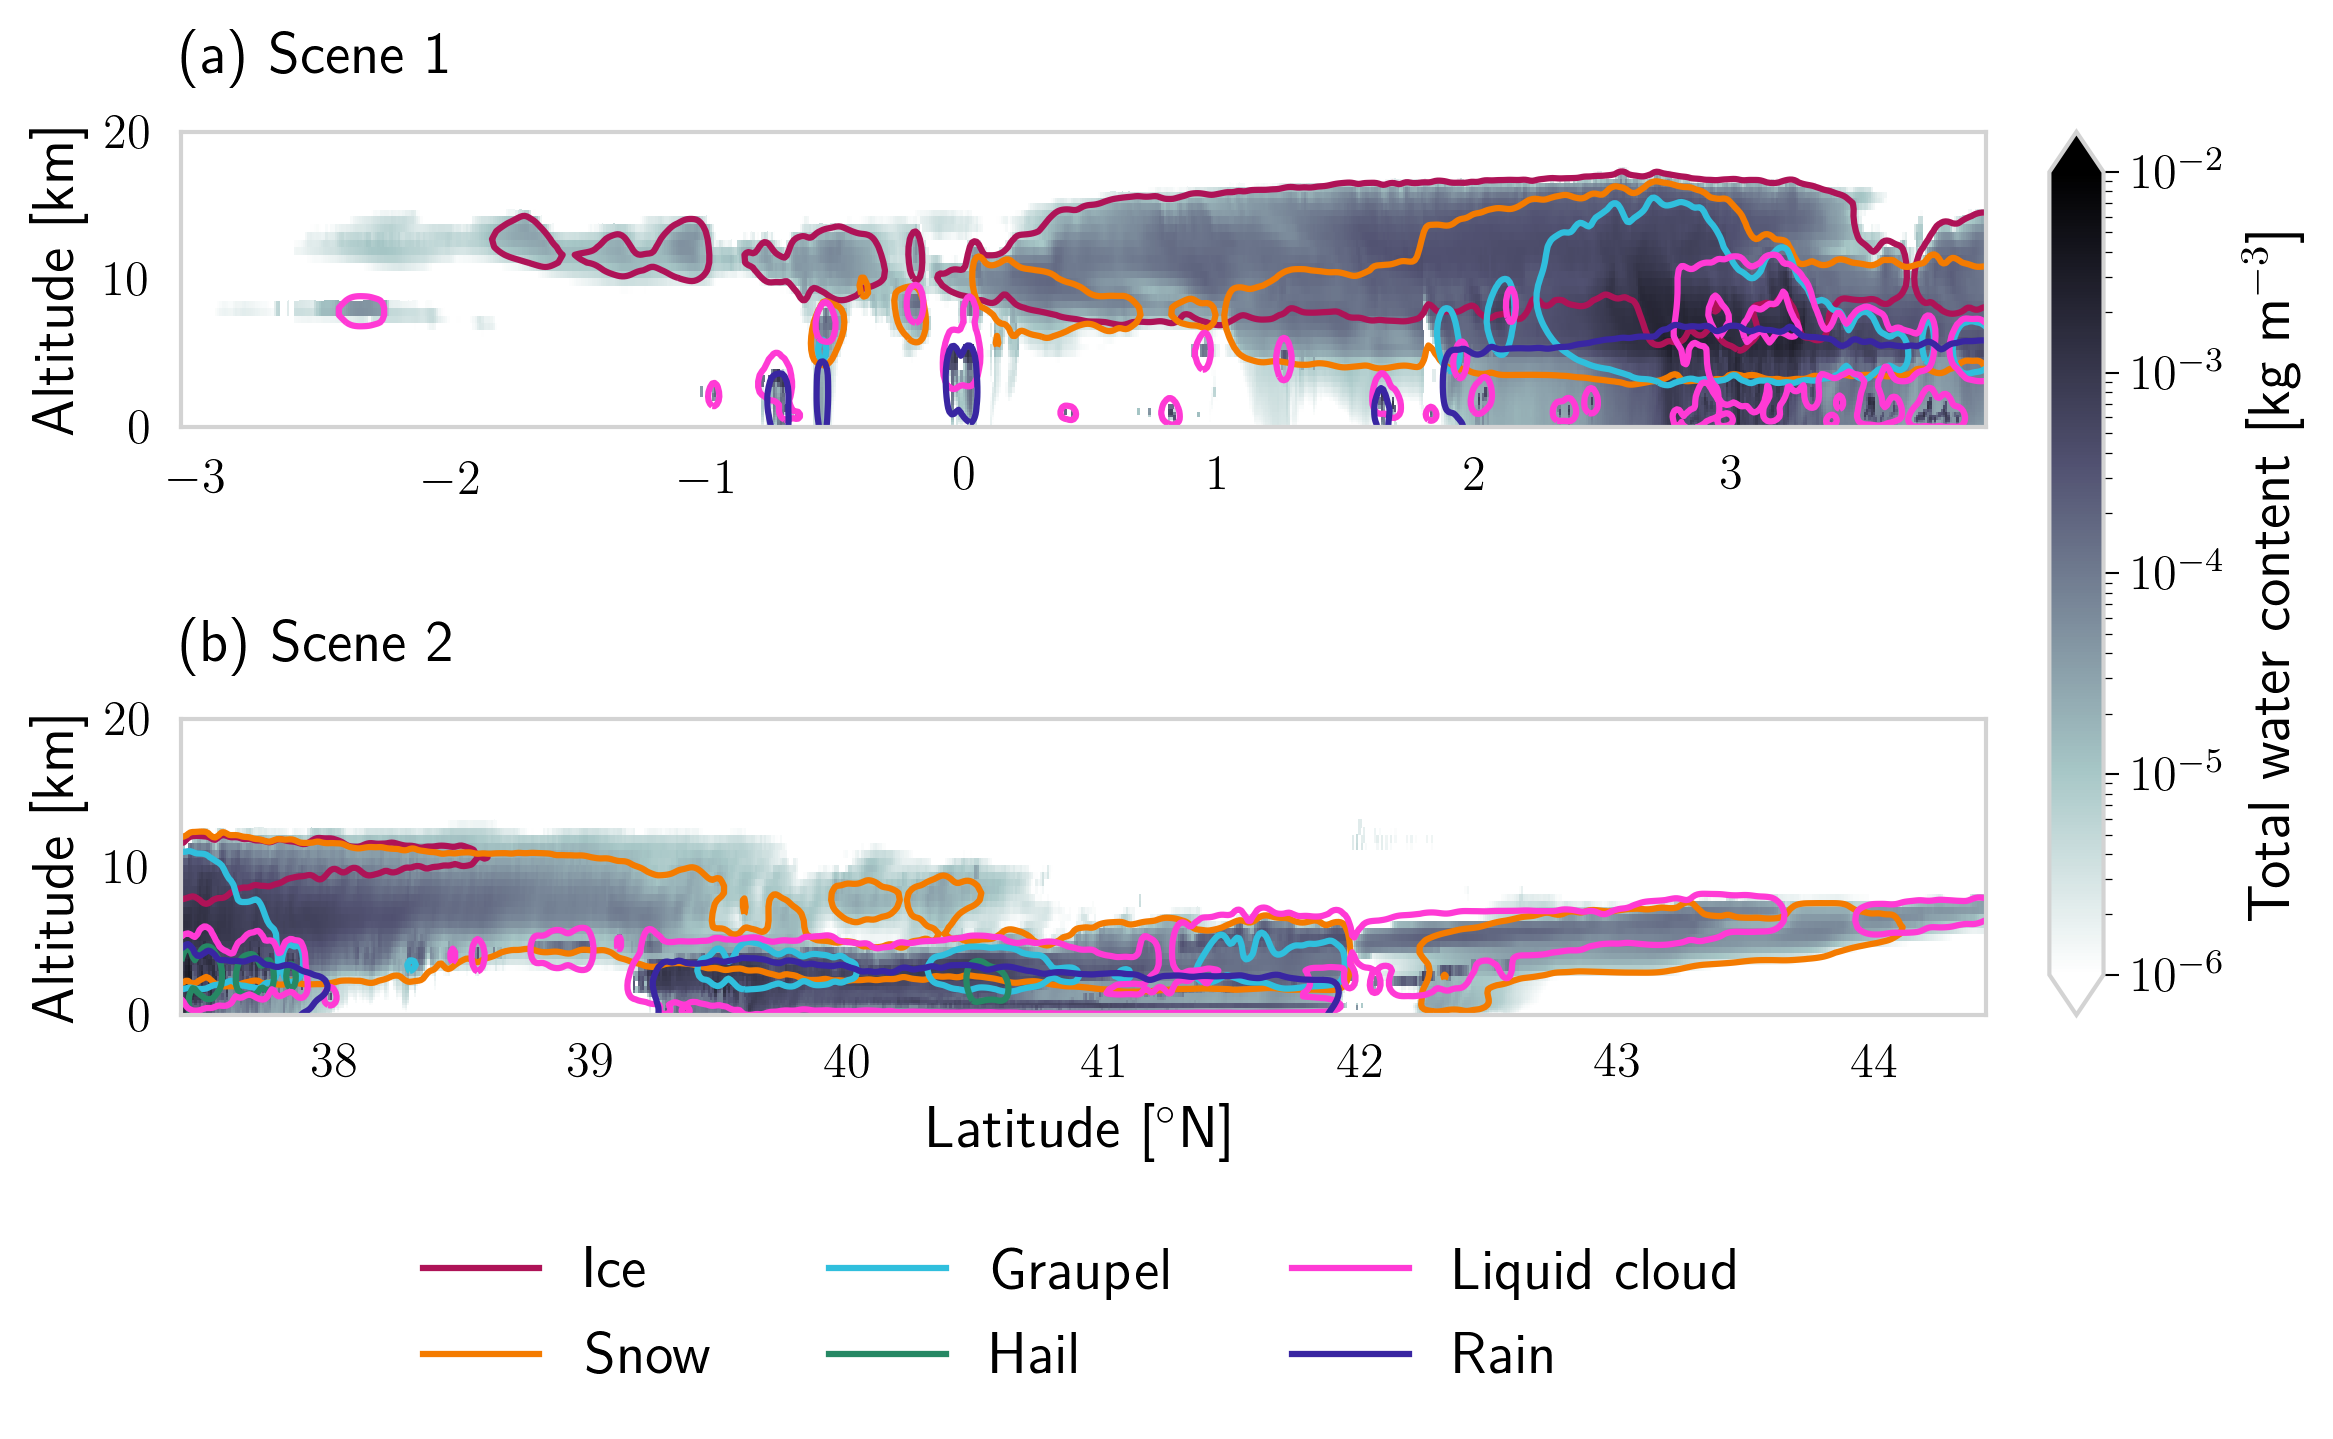
\includegraphics[width = 0.8\textwidth]{../plots/scene_overview.png}
\caption{The distribution of total water content including all hydrometeor
  classes in the two cloud scenes used to test the retrieval. Colored lines show the
 $\unit{kg\ m^{-3}}$ contour of the water content of each hydrometeor class.}
\label{fig:overview}
\end{figure}

The GEM model uses a two-moment scheme with six types of hydrometeors to
represent clouds and precipitation \citep{milbrandtyau05}: Two classes of liquid
hydrometeors (rain and liquid cloud) and four of frozen hydrometeors (cloud ice,
snow, hail and graupel). The particle size distribution (PSD) of each
hydrometeor class is described by a three-parameter gamma distribution. The
prognostic parameters of the model are the slope and intercept parameters of the
PSD, which are derived from the predicted mixing ratios and number
concentrations. The third parameter, which defines the shape of the PSD, is set
to a fixed, species-specific value. For each hydrometeor species a specific
mass-size relationship is assumed.

Examples of particle size distributions of frozen hydrometeors are displayed in
Fig.~\ref{fig:gem_psds}. The assumed particle size distributions across
different ice species vary mostly in their scaling with respect to size and
concentration, whereas the normalized shape shows less variability. Furthermore,
an important characteristic of the model can be identified here, which will help
to better understand the retrieval results presented later: Cloud ice in the
model is characterized by high particle number concentrations and small particle
sizes, whereas snow has lower number concentrations and larger particles.


\begin{figure}[h!]
\centering 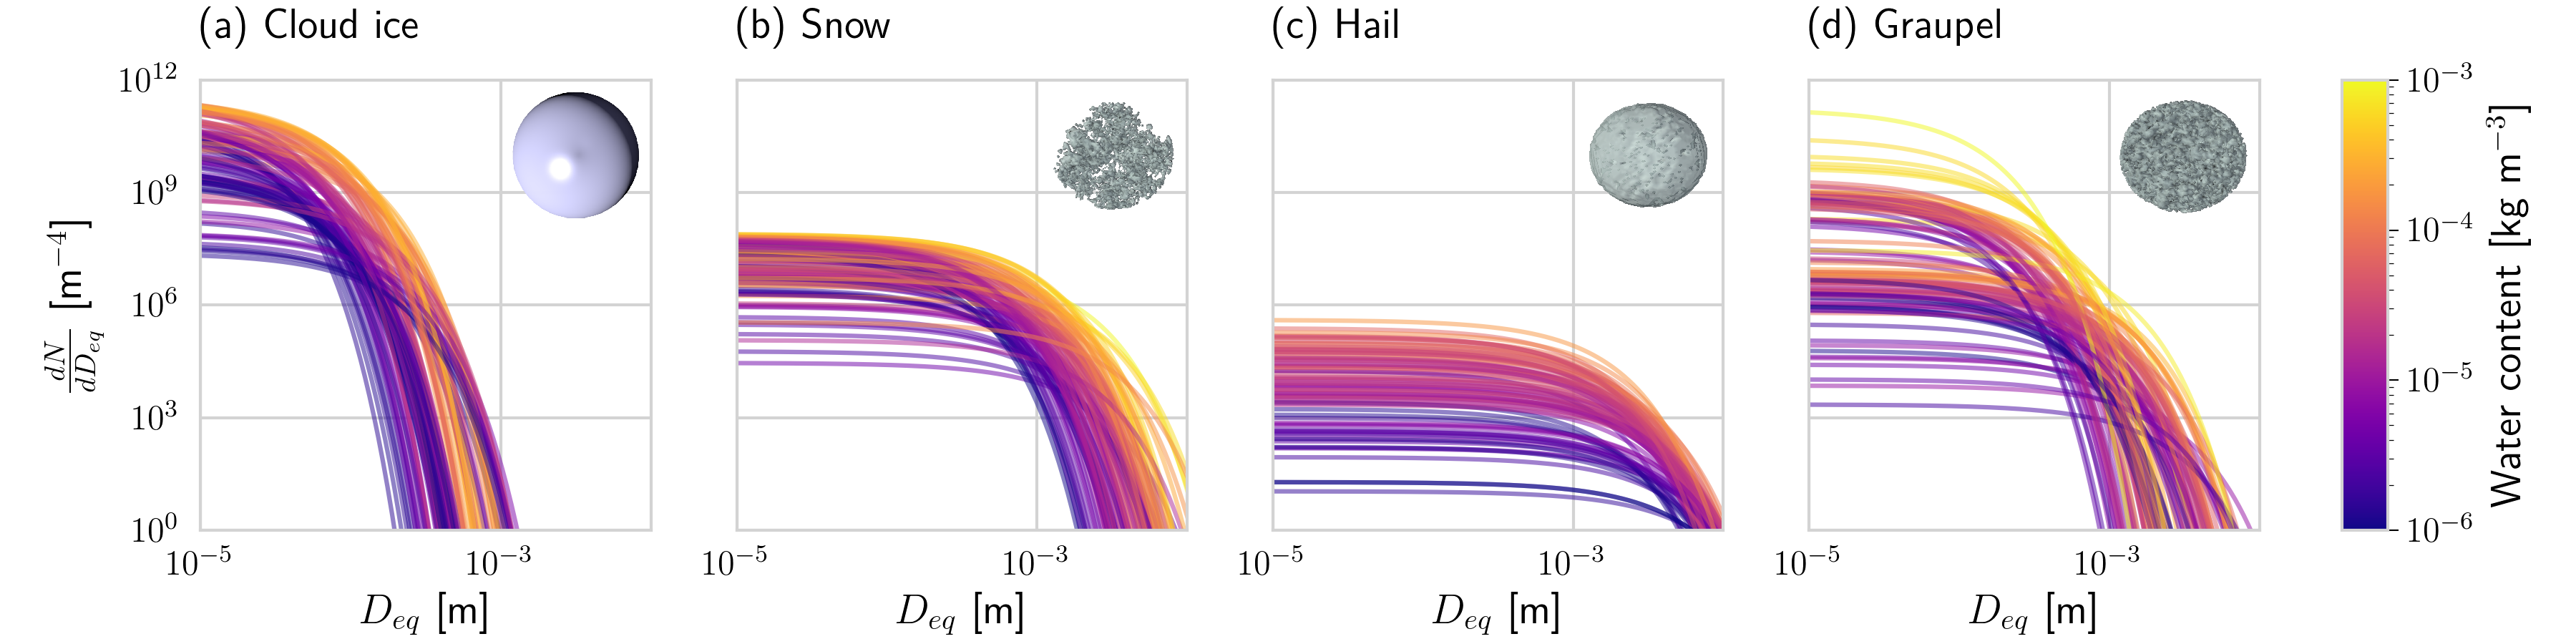
\includegraphics[width = \textwidth]{../plots/gem_psds.png}
\caption{Realizations of particle size distributions from the test scenes used
  in this study. The particle number concentration is plotted with respect to the
  volume-equivalent diameter $D_\text{eq}$. Shown are the PSDs corresponding to
  100 randomly chosen grid points with a water content higher than
  $10^{-6}\ \unit{kg\ m^{-3}}$. Line color encodes the corresponding water content.}
\label{fig:gem_psds}
\end{figure}

In order to simulate observations from the GEM model scenes, the hydrometeor
classes of the GEM microphysics scheme must be associated with particle shapes
to define their radiometric properties. The ARTS single-scattering database,
described in more detail below, contains particle models which were designed to
be consistent with the mass-size relationships assumed in the GEM model. The
particle shapes used to represent the GEM model's different hydrometeor types
are listed together with their properties in
Tab.~\ref{tab:gem_particle_properties}.

\begin{table}
  \centering
  \caption{Particle shapes used to represent the hydrometeor species of the
  GEM model scenes. The mass size relationship is given in terms of the parameters
  of a fitted power law of the form $m = \alpha \cdot D_\text{max}^\beta$.}
  \begin{tabular}{l|l|rr|rr}
    \multicolumn{1}{c|}{GEM hydrometeor class} & \multicolumn{1}{c|}{Associated particle shape}  & \multicolumn{2}{c|}{Size range} & \multicolumn{2}{c}{Mass size relationship} \\
    & Name (ID) &$D_{\text{eq}, \text{ min}}\ [\unit{\mu m}$] & $D_{\text{eq}, \text{ max}}\ [\unit{\mu m}]$ &\hfill $\alpha\ [\unit{kg\ m^{-3}}]$ & \hfill $\beta\ [\ ]$ \\
    \hline
    Liquid cloud & LiquidSphere (25) & $1$ & $5\cdot10^{4}$ & 480 & 3 \\
    Rain         & LiquidSphere (25) & $1$ & $5\cdot10^{4}$ & 480 & 3 \\
    Ice cloud    & GEM Cloud Ice (31) & $10$  & $3\cdot 10^3$    &  440 & 3 \\
    Snow    & GEM Snow (32) & $94$  & $5\cdot 10^3$    &  24 & 2.86 \\
    Graupel    & GEM Graupel (33) & $94$  & $5\cdot 10^3$    &  170 & 2.96 \\
    Hail     & GEM Hail (34) & $94$  & $5\cdot 10^3$    &  540 & 3.02 \\
  \end{tabular}
  \label{tab:gem_particle_properties}
\end{table}

\subsection{Simulated cloud observations}

An airborne sensor configuration is assumed to simulate observations. The beams
of all three sensors are assumed to point at nadir and to be perfectly
coincident pencil beams. Multiple scattering effects in the radar observations
as well as the effects of particle orientation are neglected. Although these
assumptions may be justified for an airborne configuration, this will not be the
case for space-borne observations from ICI and MWI. Moreover, the incidence
angles of the beams of ICI and MWI will be around $53^\circ$ at the Earth's
surface. This further complicates the radiative transfer modeling since it
requires treating a more complex co-location geometry of the nadir-pointing
radar and the passive instruments. At off-nadir viewing angles, polarization
also needs to be taken into account, the effects of which can be several Kelvin
at typical viewing angles of imaging sensors \citep{xie15}.

\subsubsection{Sensor configuration}
\label{sec:sensors}
The sensor configuration assumed for the simulated observations includes the 11
highest-frequency channels of the MWI radiometer and all ICI channels. For the
radar, a nadir-pointing W-band cloud radar with similar characteristics as the
CloudSat Cloud Profiling Radar (CPR, \citet{stephens02,tanelli08}) is assumed.

Observations from the ICI radiometer are simulated by performing a single,
non-polarized radiative transfer simulation located at the centers of the pass
bands of each double-sideband channel and averaging the resulting brightness
temperatures. For channels with multiple polarizations, only a single simulation
is performed. To compensate for this, the noise of the corresponding channel is
reduced by a factor of $\sqrt{2}$. The simulated ICI channels and assumed noise
levels are presented in Tab.~\ref{tab:channels}.

Observations from the MWI radiometer are simulated in a similar manner to those
of ICI except that for MWI only channels with frequencies larger than or equal
to $89\ \unit{GHz}$ are used. The reason for this is that the footprints of the
channels with frequencies lower than $89\ \unit{GHz}$ will have full-width at
half maximum of $50\ \unit{km}$ compared to only $10\ \unit{km}$ for the MWI's
higher-frequency channels and $16\ \unit{km}$ for ICI's channels. For a
spaceborne configuration, these channels were deemed unlikely to be beneficial
for a synergistic retrieval due to the very small  overlap of the
footprints of these channels with that of the radar. The included MWI channels
are listed in Tab.~\ref{tab:channels}.

\begin{table}[hbpt]
\caption{Channels of the MWI and ICI radiometers used in the retrieval.}
\label{tab:channels}
    \begin{tabular}{c|r|r|p{2cm}}
    \multicolumn{3}{c}{MWI}\\
    Channel & Freq. [GHz] & Noise [K] \\
    \hline
    MWI-8  & $89$              & $1.1$ \\
    MWI-9  & $118.75 \pm 3.2$  & $1.3$ \\
    MWI-10 & $\pm 2.1$         & $1.3$ \\
    MWI-11 & $\pm 1.4$         & $1.3$ \\
    MWI-12 & $\pm 1.2$         & $1.3$ \\
    MWI-13 & $165.5 \pm 0.75$  & $1.3$ \\
    MWI-14 & $183.31 \pm 7.0$  & $1.2$ \\
    MWI-15 & $ \pm 6.1$        & $1.2$ \\
    MWI-16 & $ \pm 4.9$        & $1.2$ \\
    MWI-17 & $ \pm 3.4$        & $1.2$ \\
    MWI-18 & $ \pm 2.0$        & $1.3$ \\
    \end{tabular}%
    \hspace{1cm}%
    \begin{tabular}{c|r|r}
    \multicolumn{3}{c}{ICI}\\
    Channel & Freq. [GHz] & Noise [K]  \\
    \hline
    ICI-1  & $183.31 \pm 7.0$ & $0.8$ \\
    ICI-2  & $       \pm 3.4$ & $0.8$ \\
    ICI-3  & $       \pm 2.0$ & $0.8$ \\
    ICI-4  & $243    \pm 2.5$ & $\frac{1}{\sqrt{2}} \cdot 0.7$ \\
    ICI-5  & $325.15 \pm 9.5$ & $1.2$ \\
    ICI-6  & $       \pm 3.5$ & $1.3$ \\
    ICI-7  & $       \pm 1.5$ & $1.5$ \\
    ICI-8  & $448    \pm 7.2$ & $1.4$ \\
    ICI-9  & $       \pm 3.0$ & $1.6$ \\
    ICI-10 & $       \pm 1.4$ & $2.0$ \\
    ICI-11 & $664    \pm 4.2$ & $\frac{1}{\sqrt{2}} \cdot 1.6$ \\
    \end{tabular}
\end{table}

The frequency of the the cloud radar is chosen to be $94\ \unit{GHz}$ similar to
the CloudSat CPR. The vertical resolution of the nadir-pointing radar observations
is assumed to be $500\ \unit{m}$ ranging from $0.5$ to $20\ \unit{km}$ in
altitude. The minimum sensitivity is set to be $-30\ \unit{dBZ}$ and the noise
at each range gate is modeled to be independent with standard deviation
$0.5\ \unit{dBZ}$.

\subsubsection{Radiative transfer simulations}
\label{sec:orge741b86}

All simulations presented in this study were performed using Version 2.3.1279 of
the Atmospheric Radiative Transfer Simulator (ARTS, \cite{arts18}). Radar
reflectivities are computed using ARTS' built-in single-scattering radar solver,
which provides analytic Jacobians. For the simulation of passive radiances, a
hybrid solver is used which combines the DISORT \citep{disort00} scattering
solver with the ARTS standard scheme for pencil beam radiative transfer. The
hybrid solver has been added to ARTS specifically for this study and provides
approximate, analytical Jacobians, which are required for  variational
retrievals of hydrometeors. All simulations are performed assuming an ocean
surface with emissivities calculated using the Tool to Estimate Sea‐Surface
Emissivity from Microwaves to sub‐Millimeter waves (TESSEM, \cite{prigent16}).
Polarization is neglected in all simulations performed in this study. Gaseous
absorption is modeled using the absorption models from \cite{rosenkranz93} for
$N_2$, $O_2$ and from \cite{rosenkranz98} for $H_2O$.

Single scattering data for hydrometeors are taken from ARTS single scattering
data base (ARTS SSDB, \citet{eriksson18}). The database provides scattering data
for a wide range of hydrometeor shapes including particles designed specifically
to be consistent with assumptions of the GEM microphysics scheme. It also
provides a number of predefined habit mixes, referred to as standard habits,
designed to cover the full range of particle sizes relevant for microwave
observations of ice hydrometeors.

\subsection{Retrieval algorithm}
\label{sec:orgb528563}

A one-dimensional, variational cloud retrieval algorithm is proposed which uses
the optimal estimation method (OEM, \cite{rodgers00}) to fit an atmospheric
state to given observations. The quality of a retrieved state $\hat{\mathbf{x}}$
and corresponding simulated observations $\hat{\mathbf{y}} =
\mathbf{F}(\hat{\mathbf{x}})$ is assessed using the following diagnostic
quantity:
%
\begin{align}
\chi^2_y &= \Delta \mathbf{y}^T \mathbf{S}_e^{-1} \Delta \mathbf{y}
\end{align}
%
Here, $\Delta \mathbf{y} = \mathbf{y} - \hat{\mathbf{y}}$ is the difference
between the fitted and true observations and $\mathbf{S}_e$ is the covariance
matrix describing the measurement errors. The quantity $\chi^2_y$ corresponds to
the sum of squared errors in the fitted observations weighted by the
uncertainties in each channel or range bin. It should be noted that the quantity
has no meaningful interpretation in terms of $\chi^2$-statistic for the errors
in the fitted observations since they will neither be independent (c.f.
Chapter~12 in \cite{rodgers00}) nor Gaussian due to the presence of forward
model error. The value is therefore used here solely as a heuristic to quantify
the goodness of the fit to the true observations.

\subsubsection{Measurement space}
\label{sec:orge7dc286}

The input for the synergistic retrieval is the combined observation vector
$\mathbf{y}$ consisting of the concatenated single-instrument observations from
the cloud radar and the two radiometers. Measurement errors are assumed to be
independent and Gaussian distributed with standard deviations according to the
noise characteristics given in Section \ref{sec:sensors}. For the
single-instrument retrievals the measurement vector consists only of
 observations from either the radar or the radiometers.


\subsubsection{State space}
\label{sec:method:state_space}

The proposed retrieval solves for profiles of two degrees of freedom of the PSDs
of frozen hydrometeors and rain along with profiles of relative humidity (RH)
and liquid-cloud water content (LCWC). An illustration of the retrieved
quantities and their respective retrieval grids for the combined and
single-instrument configurations of the retrieval are given in
Fig.~\ref{fig:retrieval_sketch}.

\begin{figure}
\centering 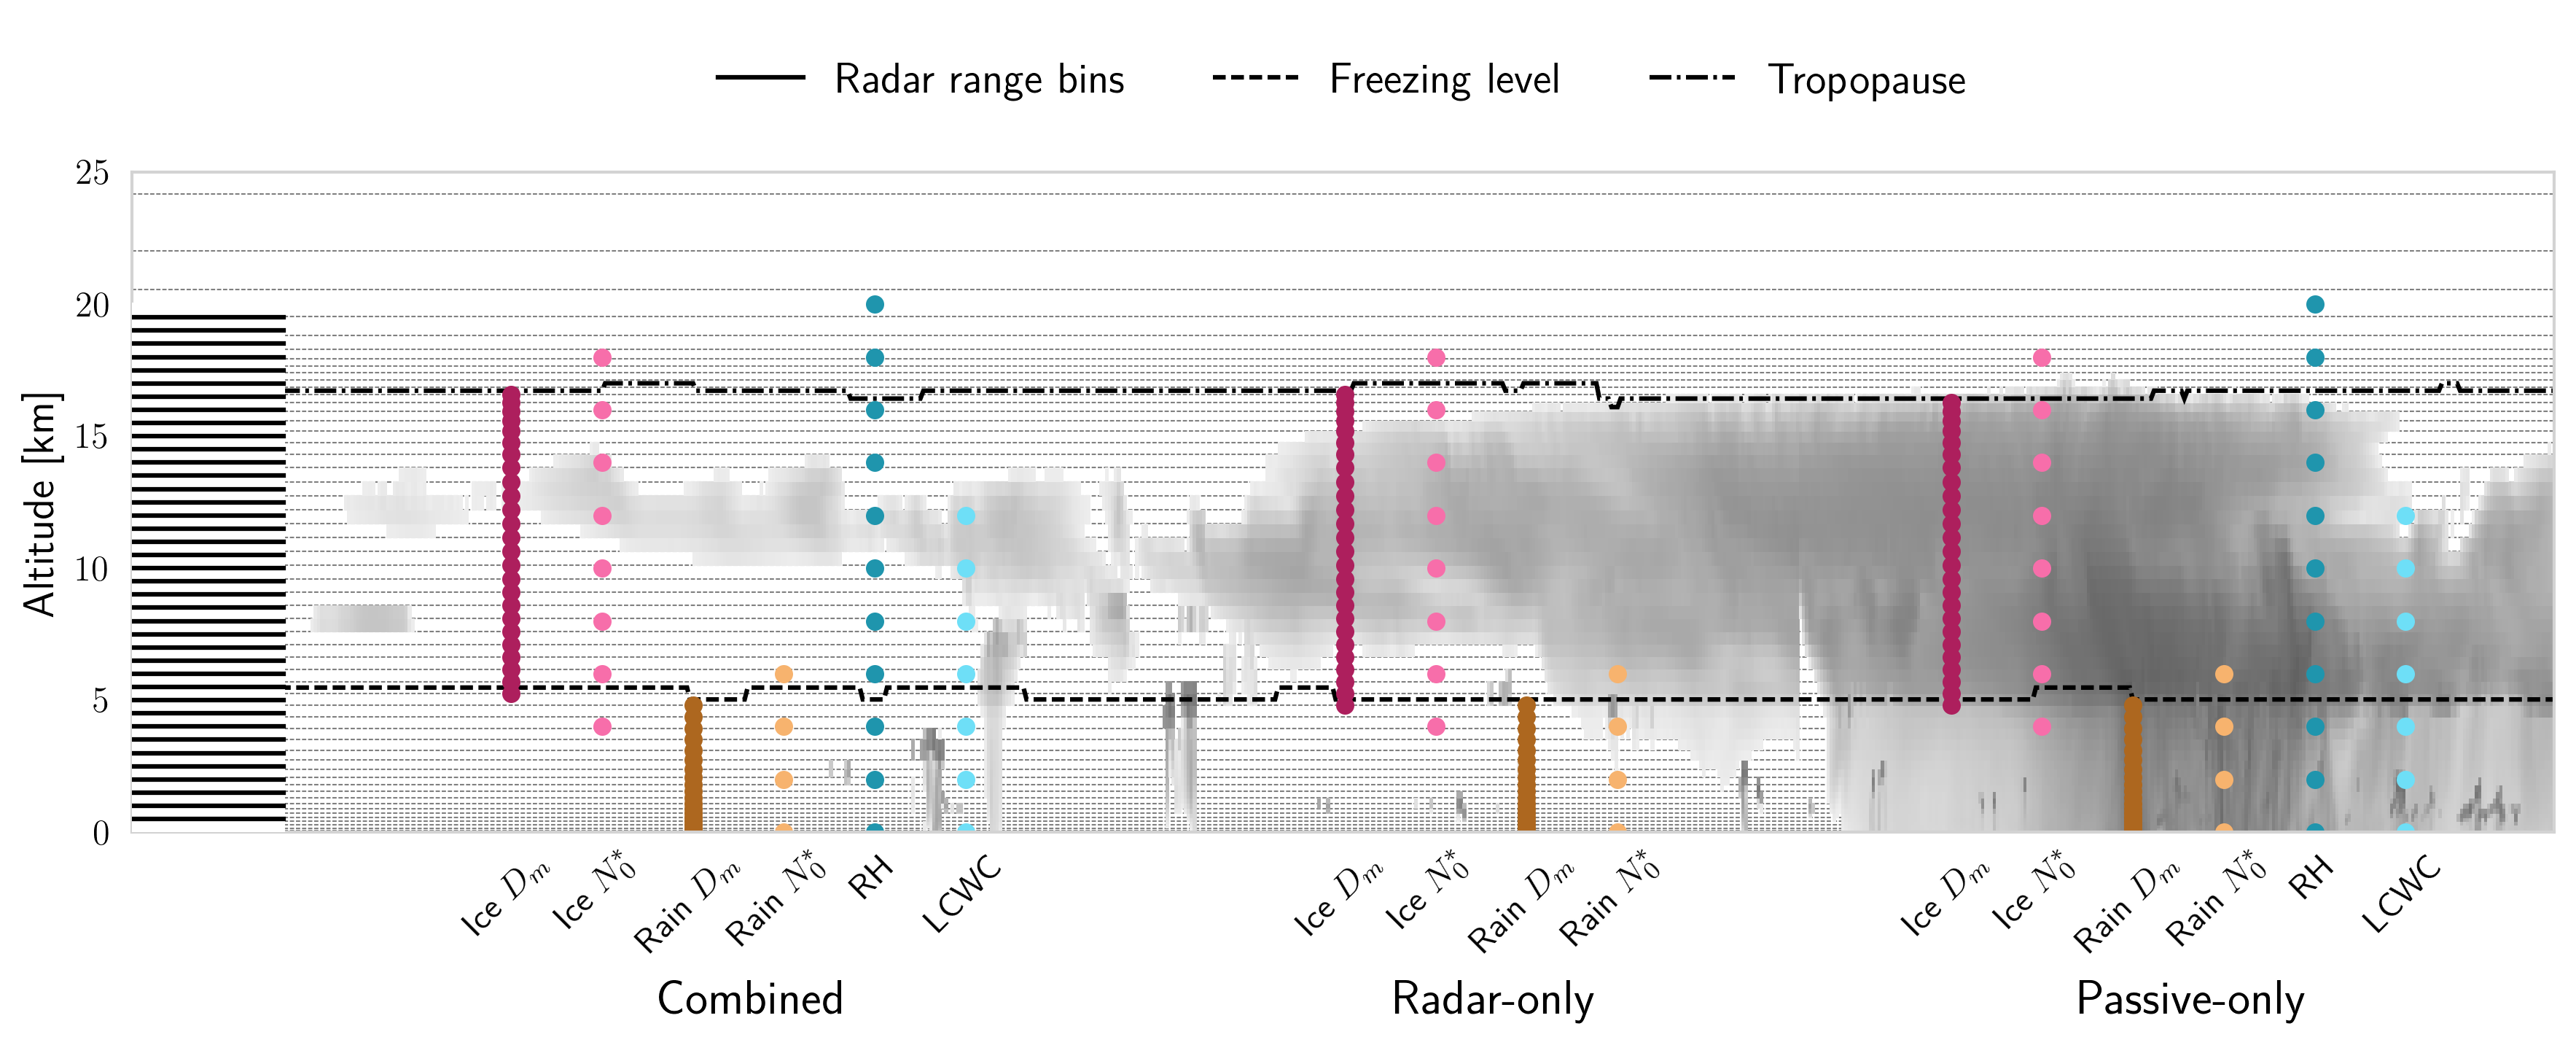
\includegraphics[width = 1.0\linewidth]{../plots/retrieval_sketch}
\caption{Illustration of retrieval quantities and their respective retrieval
  grids. Grey, dashed lines in the background display the vertical grid of the
  GEM model. Black, solid lines on the left side display the range bins of the
  radar observations. Filled markers represent the retrieval grids of each
  retrieval quantity for the combined, radar-only and passive-only
  configurations of the retrieval algorithm.}
\label{fig:retrieval_sketch}
\end{figure}

The PSDs of frozen hydrometeors and rain are represented using the normalized
particle size distribution formalism proposed by \cite{delanoe05}. The PSD of a
hydrometeor species at a given altitude is modeled using a generalized gamma
distribution function with four parameters. The mass-weighted mean diameter
$D_m$, which scales the PSD along the size dimension, and the normalized number
density $N_0^*$, which scales the particle concentration, are the two retrieved
degrees of freedom of the PSD. The other two parameters describe the shape of
the normalized PSD. The same shape parameters as in version 3 of the
DARDAR-CLOUD product \citep{cazenave19} are chosen for frozen hydrometeors. For
rain, they are chosen to match the shape used in the GEM model for rain drops.


The temperature-dependent a priori profile for $N_0^*$ for frozen hydrometeors
is determined using the relation from \cite{delanoe14}
%
\begin{align}
N_0^* &= \exp \left ( -0.076586 \cdot (T - 273.15) + 17.948 \right ),
\end{align}
%
where $T$ is in $\unit{K}$. The a priori profile of $D_m$ for frozen
hydrometeors is chosen so that the a priori IWC is equal to
$10^{-6}\ \unit{kg\ m^{-3}}$. For rain, a fixed value for $N_0^*$ of
$10^6\ \unit{m^{-4}}$ is assumed and the a priori profile for $D_m$ is
determined similarly as for frozen hydrometeors.

Since the $N_0^*$ parameters vary over several orders of magnitude they are
retrieved in $\log_{10}$-space for both frozen hydrometeors and rain. The $D_m$
parameters, in contrast, are retrieved in linear space. Alternative
parametrizations using water content and $D_m$ or the water content and $N_0^*$
have been tested but no considerable effect on retrieval performance has been
observed. As additional constraints, the retrieval of frozen hydrometeors is
restricted to the region between the freezing level, here defined simply as the
$273.15\ \unit{K}$-isotherm, and the approximate altitude of the tropopause. The
altitude of the tropopause is approximated as the first grid point at which the
lapse rate is negative and temperature below $220\ \unit{K}$. The retrieval of
rain hydrometeors is restricted to below the freezing level. The retrieval of
the $N_0^*$ parameters is further regularized by retrieving them at reduced
vertical resolution of $2\ \unit{km}$. This was found necessary to keep the
retrieval from getting stuck in spurious local minima. This resembles the
approach taken in the GPM combined precipitation retrievals \citep{grecu16},
where the PSD parameter scaling the particle concentration is also
retrieved at reduced resolution.

Relative humidity is retrieved at a vertical resolution of $2\ \unit{km}$.
However, the values are not retrieved directly but instead an inverse
hyperbolic tangent transformation is applied to the relative humidity profile:
%
\begin{align}
x = \text{arctanh}(\frac{2 \text{RH}}{1.2} - 1.0)
\end{align}
%
The transformation restricts the retrieved relative humidity values to the range
between $0$ and $120\%$. The a priori profile for relative humidity is set to
%
\begin{align}
\text{RH}(t) = \begin{cases}
 0.7 &, 270\ \unit{K} < t \\
 0.7 - 0.01 \cdot (270 -t) & ,220 < t \leq  270\ \unit{K} \\
 0.2 &,t < 220 \unit{K} \\
 \end{cases}.
\end{align}
%
LCWC is retrieved at a resolution of $2\ \unit{km}$ but is restricted to the
region between the surface and the $230\ \unit{K}$ isotherm. In contrast to
frozen hydrometeors and rain, the PSD of liquid cloud droplets is not explicitly
resolved in the retrieval forward model. Instead, liquid cloud droplets are
modeled as purely absorbing quantity using the model by \cite{liebe93} for
suspended liquid cloud droplets. Note that this is the case only for the
retrieval. For the simulated observations, liquid cloud droplets are
handled as any other hydrometeor species in the GEM model. LCWC is retrieved in
$\text{log}_{10}$-space and the a priori profile is set to a fixed value of
$10^{-6}\ \unit{kg\ m^{-3}}$ in the permitted region of the atmosphere.

The a priori distributions of the 6 retrieval quantities ($N_0^*$ and $D_m$ for
frozen and liquid hydrometeors, RH, CLWC) are assumed to be independent so that
the overall a priori covariance matrix $\mathbf{S}_a$ has block-diagonal
structure. Within each block, vertical correlations between the values of a
given retrieval quantity at different altitudes are assumed to be exponentially
decaying. The covariance of the values of retrieval quantity $q$ at
points $i$ and $j$ of the retrieval grid is computed as
%
\begin{align}
\left ( \mathbf{S}_{a,q} \right )_{i, j} &= \sigma_{q,i} \sigma_{q,j}
 \cdot \exp  \left ( -\frac{d(i, j)}{l_q} \right ),
\end{align}
%
where $\sigma_{q, i}$ is the a priori uncertainty assumed for retrieval
quantity $q$ at grid point $i$, $d(i, j)$ the distance between the grid
points and $l_q$ the quantity-specific correlation length. The assumed
a priori uncertainties and correlation lengths for the retrieval quantities
are summarized in Tab.~\ref{tab:a_priori}.

\begin{table}[h!]
\caption{A priori uncertainties and correlation
 lengths used in the retrieval.}
 \centering
\label{tab:a_priori}
    \begin{tabular}{ll|cc|cc|}
      \multicolumn{2}{c|}{Retrieval target}  & \multicolumn{2}{c|}{Combined / Radar-only} & \multicolumn{2}{c}{Passive-only}\\
      Name & Retrieved quantity &  $\sigma_q$ & $l_q$ [km] & $\sigma_q$ & $l_q$ [km]\\
    \hline
Ice, $N_0^*$ & $\log_{10}(N_{0, \text{Ice}}^*)$ & $2$ & $2$ & $2$ &$5$ \\
Ice, $D_m$ &   $\text{Ice }D_{m, \text{Ice}}$   & $300\ \unit{\mu m}$  & $2$ & $300\ \unit{\mu m}$          & $5$ \\
Rain, $N_0^*$ &    $\log_{10}(\text{Rain } N_{0}^*)$ & $2$ & $2$ & $2$ &$5$ \\
Rain, $D_m$ &  $D_{m, \text{Rain}}$   & $300\ \unit{\mu m}$  & $2$ & $300\ \unit{\mu m}$          & $5$ \\
Relative humidity (RH) & $\text{arctanh}(\frac{2 \cdot \text{RH}}{1.2} - 1.0)$ & $0.5^{*}$ & $2^{*}$ & $0.5$ & $2$ \\
Cloud liquid water content (CLWC) & $\log_{10}(\text{CLWC}) $ & $1^{*}$ & $2^{*}$  & $1$ & $2$ \\
\multicolumn{6}{l}{$^*$: Not retrieved in radar-only retrieval}
    \end{tabular}
\end{table}

The radar-only version of the retrieval is similar to the combined version
except that RH and LCWC are not retrieved. Instead, perfect knowledge of the
true RH profile is assumed while LCWC is neglected. In addition to a two-moment
radar-only retrieval, also a one-moment version (M1), in only the $D_m$
parameter is retrieved has been tested. For completeness, retrieval results for
IWC will be reported also for the M1 version. However, to allow for better
comparison with the combined and passive-only retrieval, for the remaining
results only the two-moment version is considered. For the passive-only
retrieval, the retrieval quantities and grids are the same as for the combined
retrieval. However, higher correlations lengths are assumed, which are shown in
Tab.~\ref{tab:a_priori}

\subsubsection{Representation of ice particle shape}
\label{sec:method:partilce_models}

A major difficulty for cloud retrievals is that the observations may not provide
sufficient information to distinguish different hydrometeor species. Due to this
ambiguity, frozen hydrometeors in the proposed retrieval algorithm are
represented using only a single hydrometeor species. It is therefore necessary
to find a suitable representation for frozen hydrometeors, which can capture the
variability of the four frozen hydrometeor species in the model and ideally also
that of real ice hydrometeors.

In the model scenario considered here the differences between hydrometeor
species are mostly due to their different concentrations, sizes and shape (c.f.
Fig.~\ref{fig:gem_psds}). Since two parameters of the PSD of frozen hydrometeor
species are retrieved, the retrieval can represent the different concentrations
and particle sizes characteristic for the different hydrometeor species. Changes
in particle shape from ice crystals, with typically  smaller diameters than
aggregates or rimed particles, can be represented by using a habit mix, which
combines pristine shapes at small sizes with aggregates or rimed particles at
larger sizes. This provides the retrieval with some flexibility to represent the
different shapes present in the test scenes.

It is clear that even with this configuration, the simplified retrieval forward
model will not be able to represent every possible configuration of mixes of the
four ice hydrometeor species in the GEM model. In particular, it remains unclear
which particle shape should be used to best represent this mixture. We therefore
choose a set consisting of multiple particle shapes and habit mixes, which will
be used in the retrieval to study the impact of the choice of the particle shape
on the retrieval results. The selected particles are listed in
Tab.~\ref{tab:particle_properties}. Three of them, GEM Cloud Ice, GEM Snow, and
GEM Graupel, correspond to the shapes present in the GEM model scenes. The GEM
Snow and Graupel habits were mixed with crystal shapes to ensure that they cover
sizes down to around $10\ \unit{\mu m}$. In addition to this, two of the habit
mixes distributed with the ARTS SSDB, the Large Plate Aggregate and Large Column
Aggregate standard habits, are added to the selection to increase the range of
scattering properties covered. Fig.~\ref{fig:particle_properties} provides an
overview of the bulk backscattering and extinction efficiencies of the 
particle selection computed for three different values of the $N_0^*$ parameter
of the PSD. The backscattering and extinction efficiencies are defined as
the ratio of the corresponding cross-section $\sigma$ and the bulk-mass $m$:
\begin{align}
  Q &= \frac{\sigma}{m}
\end{align}
For high values of $N_0^*$, which are typical for cloud ice, the radiometric
properties of particle shapes differ only for large masses at the two highest
frequencies considered. For low $N_0^*$ values, which are more typical for snow,
the particles' properties differ considerably at all masses and frequencies. At
the two lowest frequencies, the Large Column Aggregate, Large Plate Aggregate
and GEM Snow are the least efficient in scatterers or absorbers of radiation
whereas GEM Graupel, Gem Hail and GEM Cloud Ice are more efficient. This behavior
is also observed at the two higher frequencies, except for the lowest $N_0^*$
value for which a reversal of the ordering occurs as the bulk mass increases.

\begin{table}
  \centering
  \caption{Particle models used to represent ice hydrometeors used in the
    retrieval. The mass size relationship is given in terms of the parameters
  of a fitted power law of the form $m = \alpha \cdot D_\text{max}^\beta$.}
  \begin{tabular}{l|l|rr|rr}
    \multicolumn{1}{c|}{Name} & \multicolumn{1}{c|}{Shapes used} &
    \multicolumn{2}{c|}{Size range} & \multicolumn{2}{c}{Mass size relationship}
    \\
    & Name (ID) &$D_{\text{eq}, \text{ min}}\ [\unit{\mu m}$] &
    $D_{\text{eq}, \text{ max}}\ [\unit{\mu m}]$ &\hfill
    $\alpha\ [\unit{kg\ m^{-3}}]$ & \hfill $\beta\ [\ ]$ \\
    \hline \hline % GEM
    CloudIce & GEM CloudIce (11) & $10\ $ & $3000\ $ & \hfill 440 & \hfill 3 \\
    %
    %
    % GEM Snow
    %
    \hline GEM Snow & Evans Snow Aggregate (1) & $10\ $ & $127\ $ & \hfill 440 &
    \hfill 3 \\ & GEM Snow (32) & $107\ $ & $5000\ $ & \hfill 24 & \hfill 2.86
    \\
    %
    % Gem Graupel
    %
    \hline GEM Graupel & 8-Column Aggregate(8) & $10\ $ & $179\ $ & \hfill 65 &
    \hfill 3 \\ & GEM Graupel (33) & $107\ $ & $5000\ $ & \hfill 170 & \hfill
    2.96 \\
    %
    % Large Plate Aggregate
    %
    \hline Large Plate Aggregate & Thick Plate (15) & $16\ $ & $200\ $ & \hfill
    110 & \hfill 3 \\ & Large Plate Aggregate (33) & $160\ $ & $3021\ $ & \hfill
    0.21 & \hfill 2.26 \\
    %
    % Large Column Aggregate
    %
    \hline Large Column Aggregate & Block Column (12) & $10\ $ & $200\ $ &
    \hfill 110 & \hfill 3 \\ & Large Column Aggregate (22) & $160\ $ & $3021\ $
    & \hfill 0.25 & \hfill 2.43 \\
  \end{tabular}
  \label{tab:particle_properties}
\end{table}

\begin{figure}
  \centering
  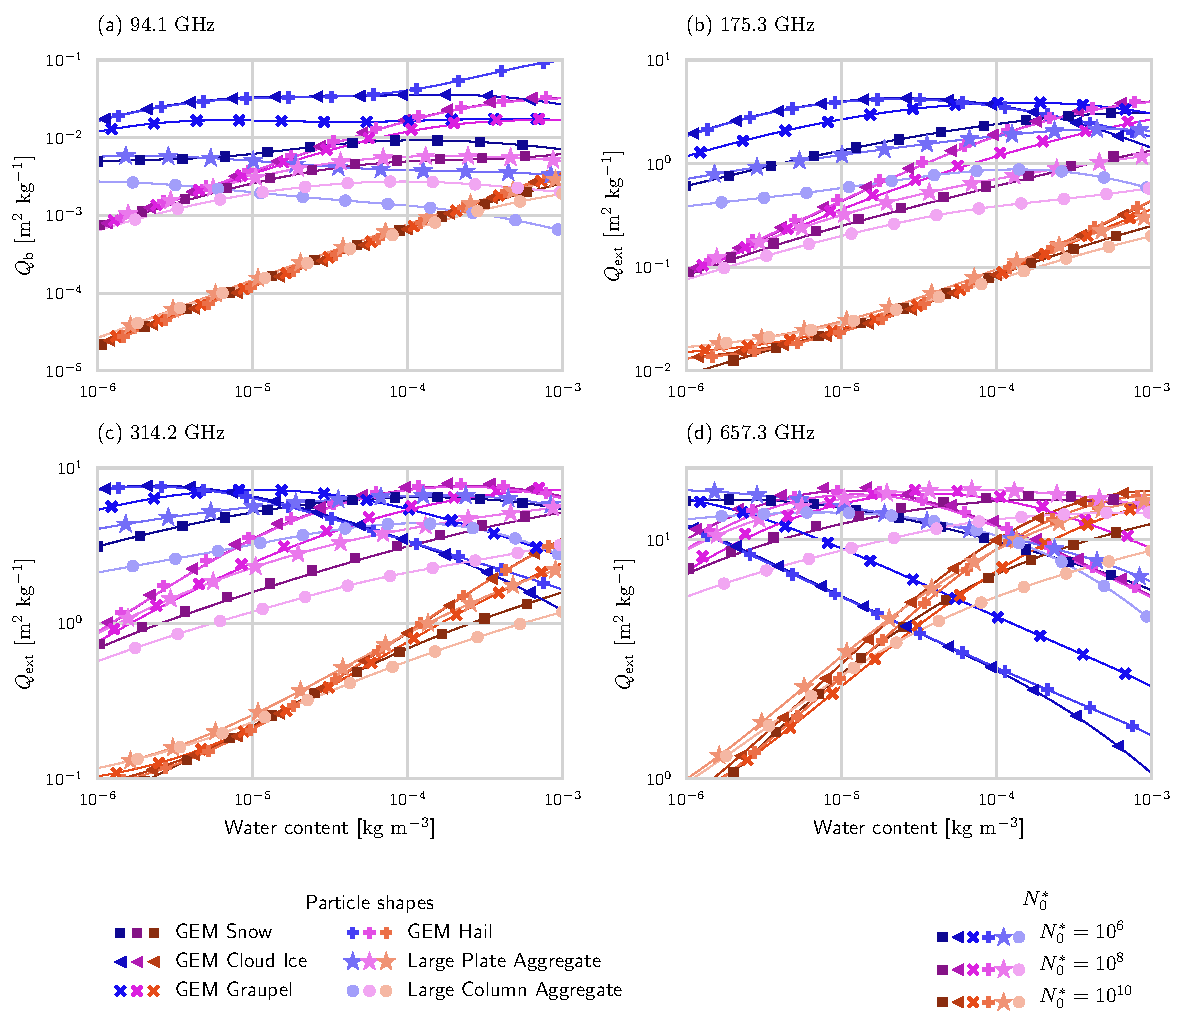
\includegraphics[width=0.8\textwidth]{../plots/particle_properties_d14}
  \caption{Bulk backscattering efficiency $Q_b$ at $94.1\ \unit{GHz}$ (a) and
    bulk extinction efficiencies $Q_{e}$ at frequencies
    $175.3\ \unit{GHz}$ (b), $314.2\ \unit{GHz}$ (c) and
    $657.3\ \unit{GHz}$ (d) for the particle models used in the simulated
    observations and the retrieval. Different colors show the bulk properties
    for different values of the $N_0^*$ parameter of the PSD.}
  \label{fig:particle_properties}
\end{figure}

\section{Results}
\label{sec:results}

The first part of this section presents results from a numerical experiment which
investigates the complementary information content of the active and passive
microwave observations. Results of the combined and the single-instrument
retrievals applied to the reference cloud scenes are presented in the second
part.

\subsection{Complementary information content}
\label{sec:simple_cloud}

A fundamental question regarding the benefit of combining two remote sensing
observations in a retrieval is to what extent the observations contain
non-redundant information. The degree of non-redundancy in the combined
observations is what we refer to here as complementary information content. We
are thus interested in the information that cannot be provided by either of the
instruments alone. Because of this, the higher resolution achieved by adding
radar observations to passive ones is not considered as complementary
information since the radar alone can provide the increased resolution.

In order to explore the complementary information content in the radar and
radiometer observations, an idealized, homogeneous cloud layer with a thickness
of $5\ \unit{km}$ centered at an altitude of $10\ \unit{km}$ in a tropical
atmosphere is considered. The cloud is assumed to consist of a single species of
frozen hydrometeors represented using the PSD parametrization which is also used
in the retrieval and described in Sec.~\ref{sec:method:state_space}. As particle
model, the 8-Column Aggregate (ID 8) from the ARTS SSDB is used.

The question that is addressed here is whether the combination of active and
passive observations is able to constrain both the size and concentration of the
ice particles in the cloud. To investigate this, the $N_0^*$ and $D_m$
parameters of the homogeneous cloud layer are varied and observations of the
cloud are simulated. The cloud signal in the radiometer observations is the
difference between the cloudy- and clear-sky brightness temperatures ($\Delta
T_B$). The signal in the active observations is here defined as the maximum of
the measured profile of radar reflectivity $\text{dBZ}_\text{max}$.
Figure~\ref{fig:contours} displays the contours of $\Delta T_B$ and
$\text{dBZ}_\text{max}$ with respect to $D_m$ and the cloud's water content,
which is proportional to $N_0^*$:
\begin{align}
m = \frac{\pi \rho}{4 ^ 4}N_0^* D_m^4,
\end{align}
with $\rho$ the density of ice.

\begin{figure}
\centering
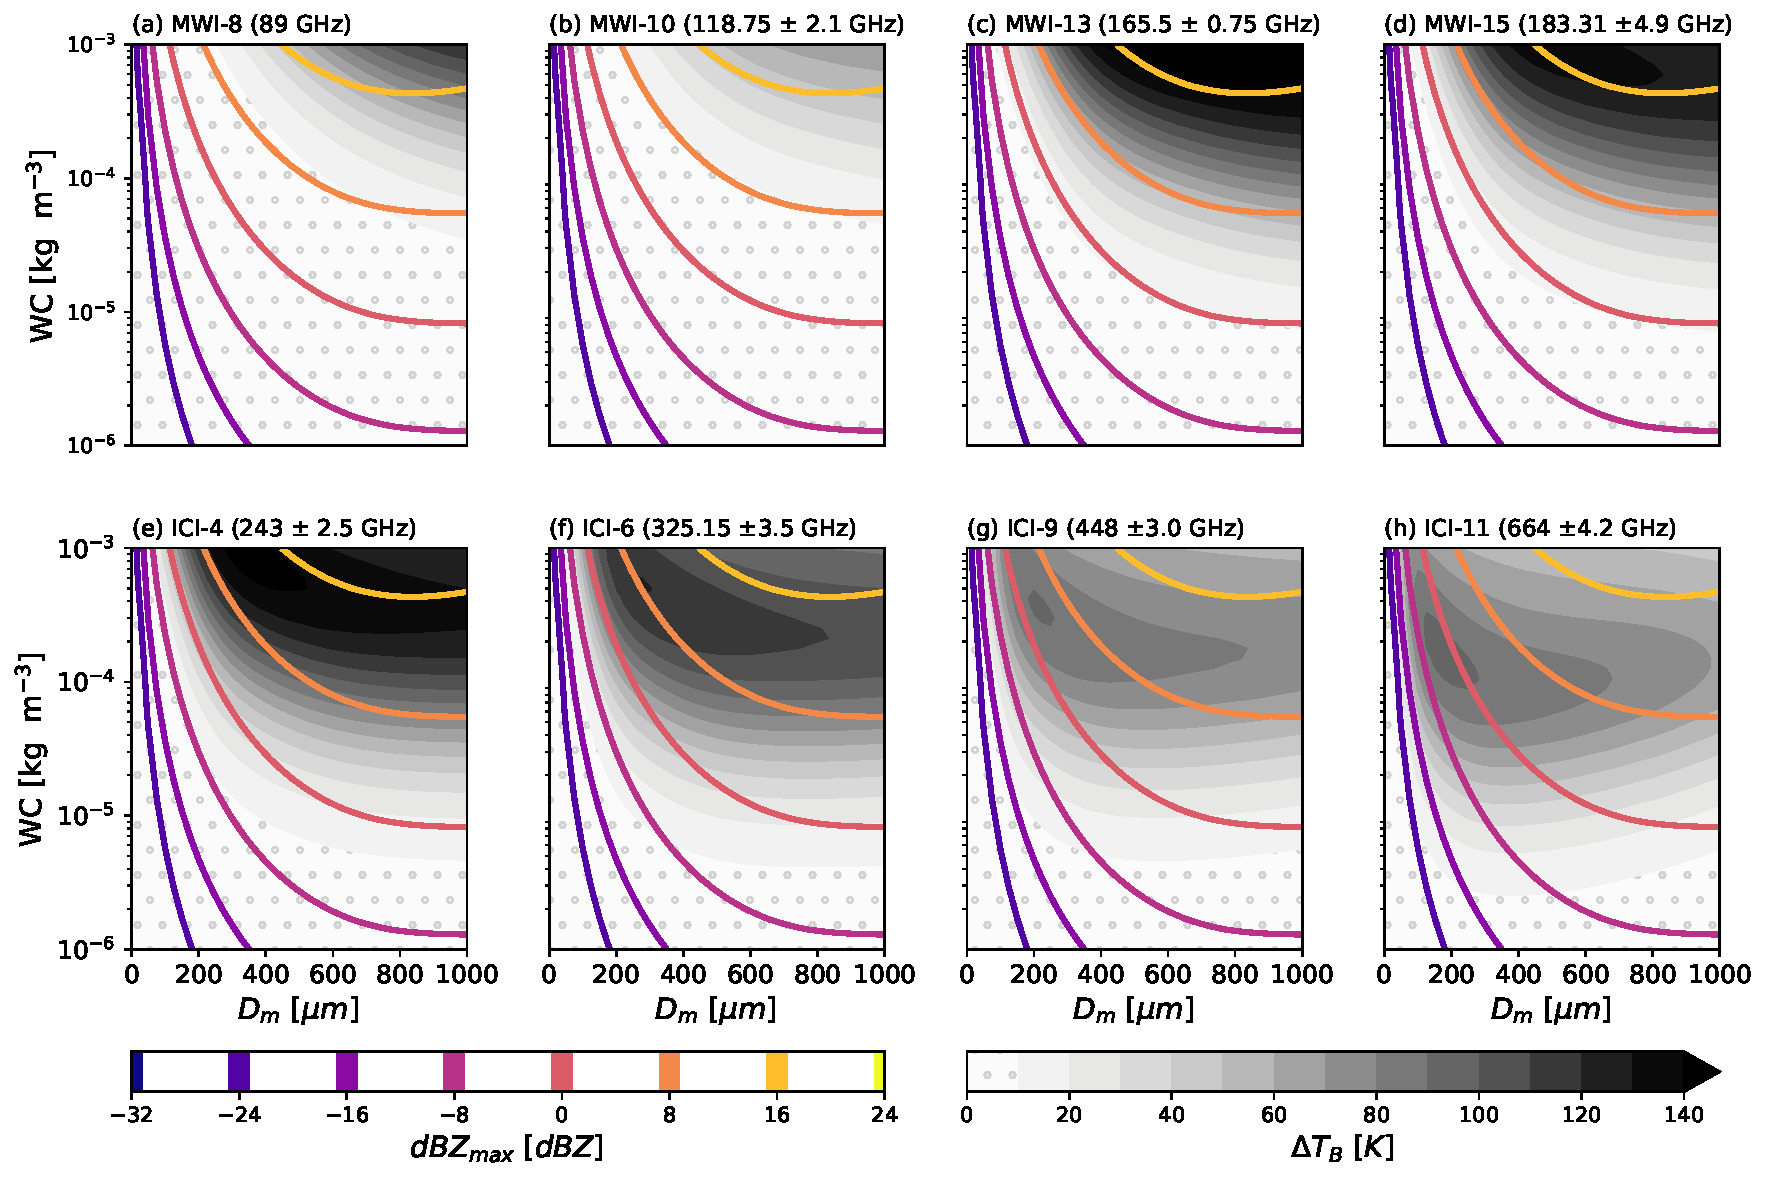
\includegraphics[width = 1.0\textwidth]{../plots/contours}
\caption{Simulated observations of a homogeneous, $5\ \unit{km}$ thick cloud
  layer with varying water content $m$ and mass-weighted mean diameter $D_m$.
  The panels display the maximum radar reflectivity in dBZ
  ($\text{dBZ}_\text{max}$) overlaid onto the cloud signal ($\Delta T_B$)
  measured by selected radiometer channels of the MWI (first row) and ICI
  radiometers (second row).}
\label{fig:contours}
\end{figure}

Along the $\text{dBZ}_\text{max}$-contours the cloud composition changes but the
observed signal stays the same. This shows the ambiguity of the radar
observations with respect to the cloud composition. A necessary condition for a
passive observation at a given frequency to be able to resolve this ambiguity is
that the contours of the active and passive signals cross each other. The panels
in Fig.~\ref{fig:contours} thus provide an indication to what extent the
information in the radar measurement and the corresponding passive radiometer
channel provide complementary information two degrees of freedom of the PSD. The
results show that the MWI channels provide complementary information only for
very dense clouds consisting with large particles. In contrast to that, the ICI
observations exhibit crossing contours already at lower water content and $D_m$
values, indicating complementary information for less dense clouds consisting of
smaller particles.

\subsection{Retrieval results}

To assess the performance of the combined cloud retrieval, the developed
algorithm has been applied to the two designated cloud scenes. The same
retrievals have been performed with a radar-only and a passive-only version of
the algorithm to serve as baselines for the evaluation of the combined
retrieval. Each retrieval was performed multiple times using the different ice
particle models listed in Tab.~\ref{tab:particle_properties}. Since the results
for both test scenes are qualitatively similar, results from the second scene
are provided in App.~\ref{app:results_b}. Complete results for all retrieval quantities,
both scenes and all tested particle shapes are provided as digital supplement to
this article.

The simulated observations which were generated to test the retrievals
are shown for the first test scene in Fig.~\ref{fig:observations_a}. Independent
Gaussian noise with standard deviations according to sensor specifications has
been added to the simulated observations to account for sensor noise. It is
important to note that the simulated observations which are used to test the
retrieval assume different microphysics than what is assumed in the retrieval.
The synthetic observations are computed using the six hydrometeor classes from
the GEM model, while the retrieval forward model assumes only two classes of
hydrometeors.

\begin{figure}
\centering 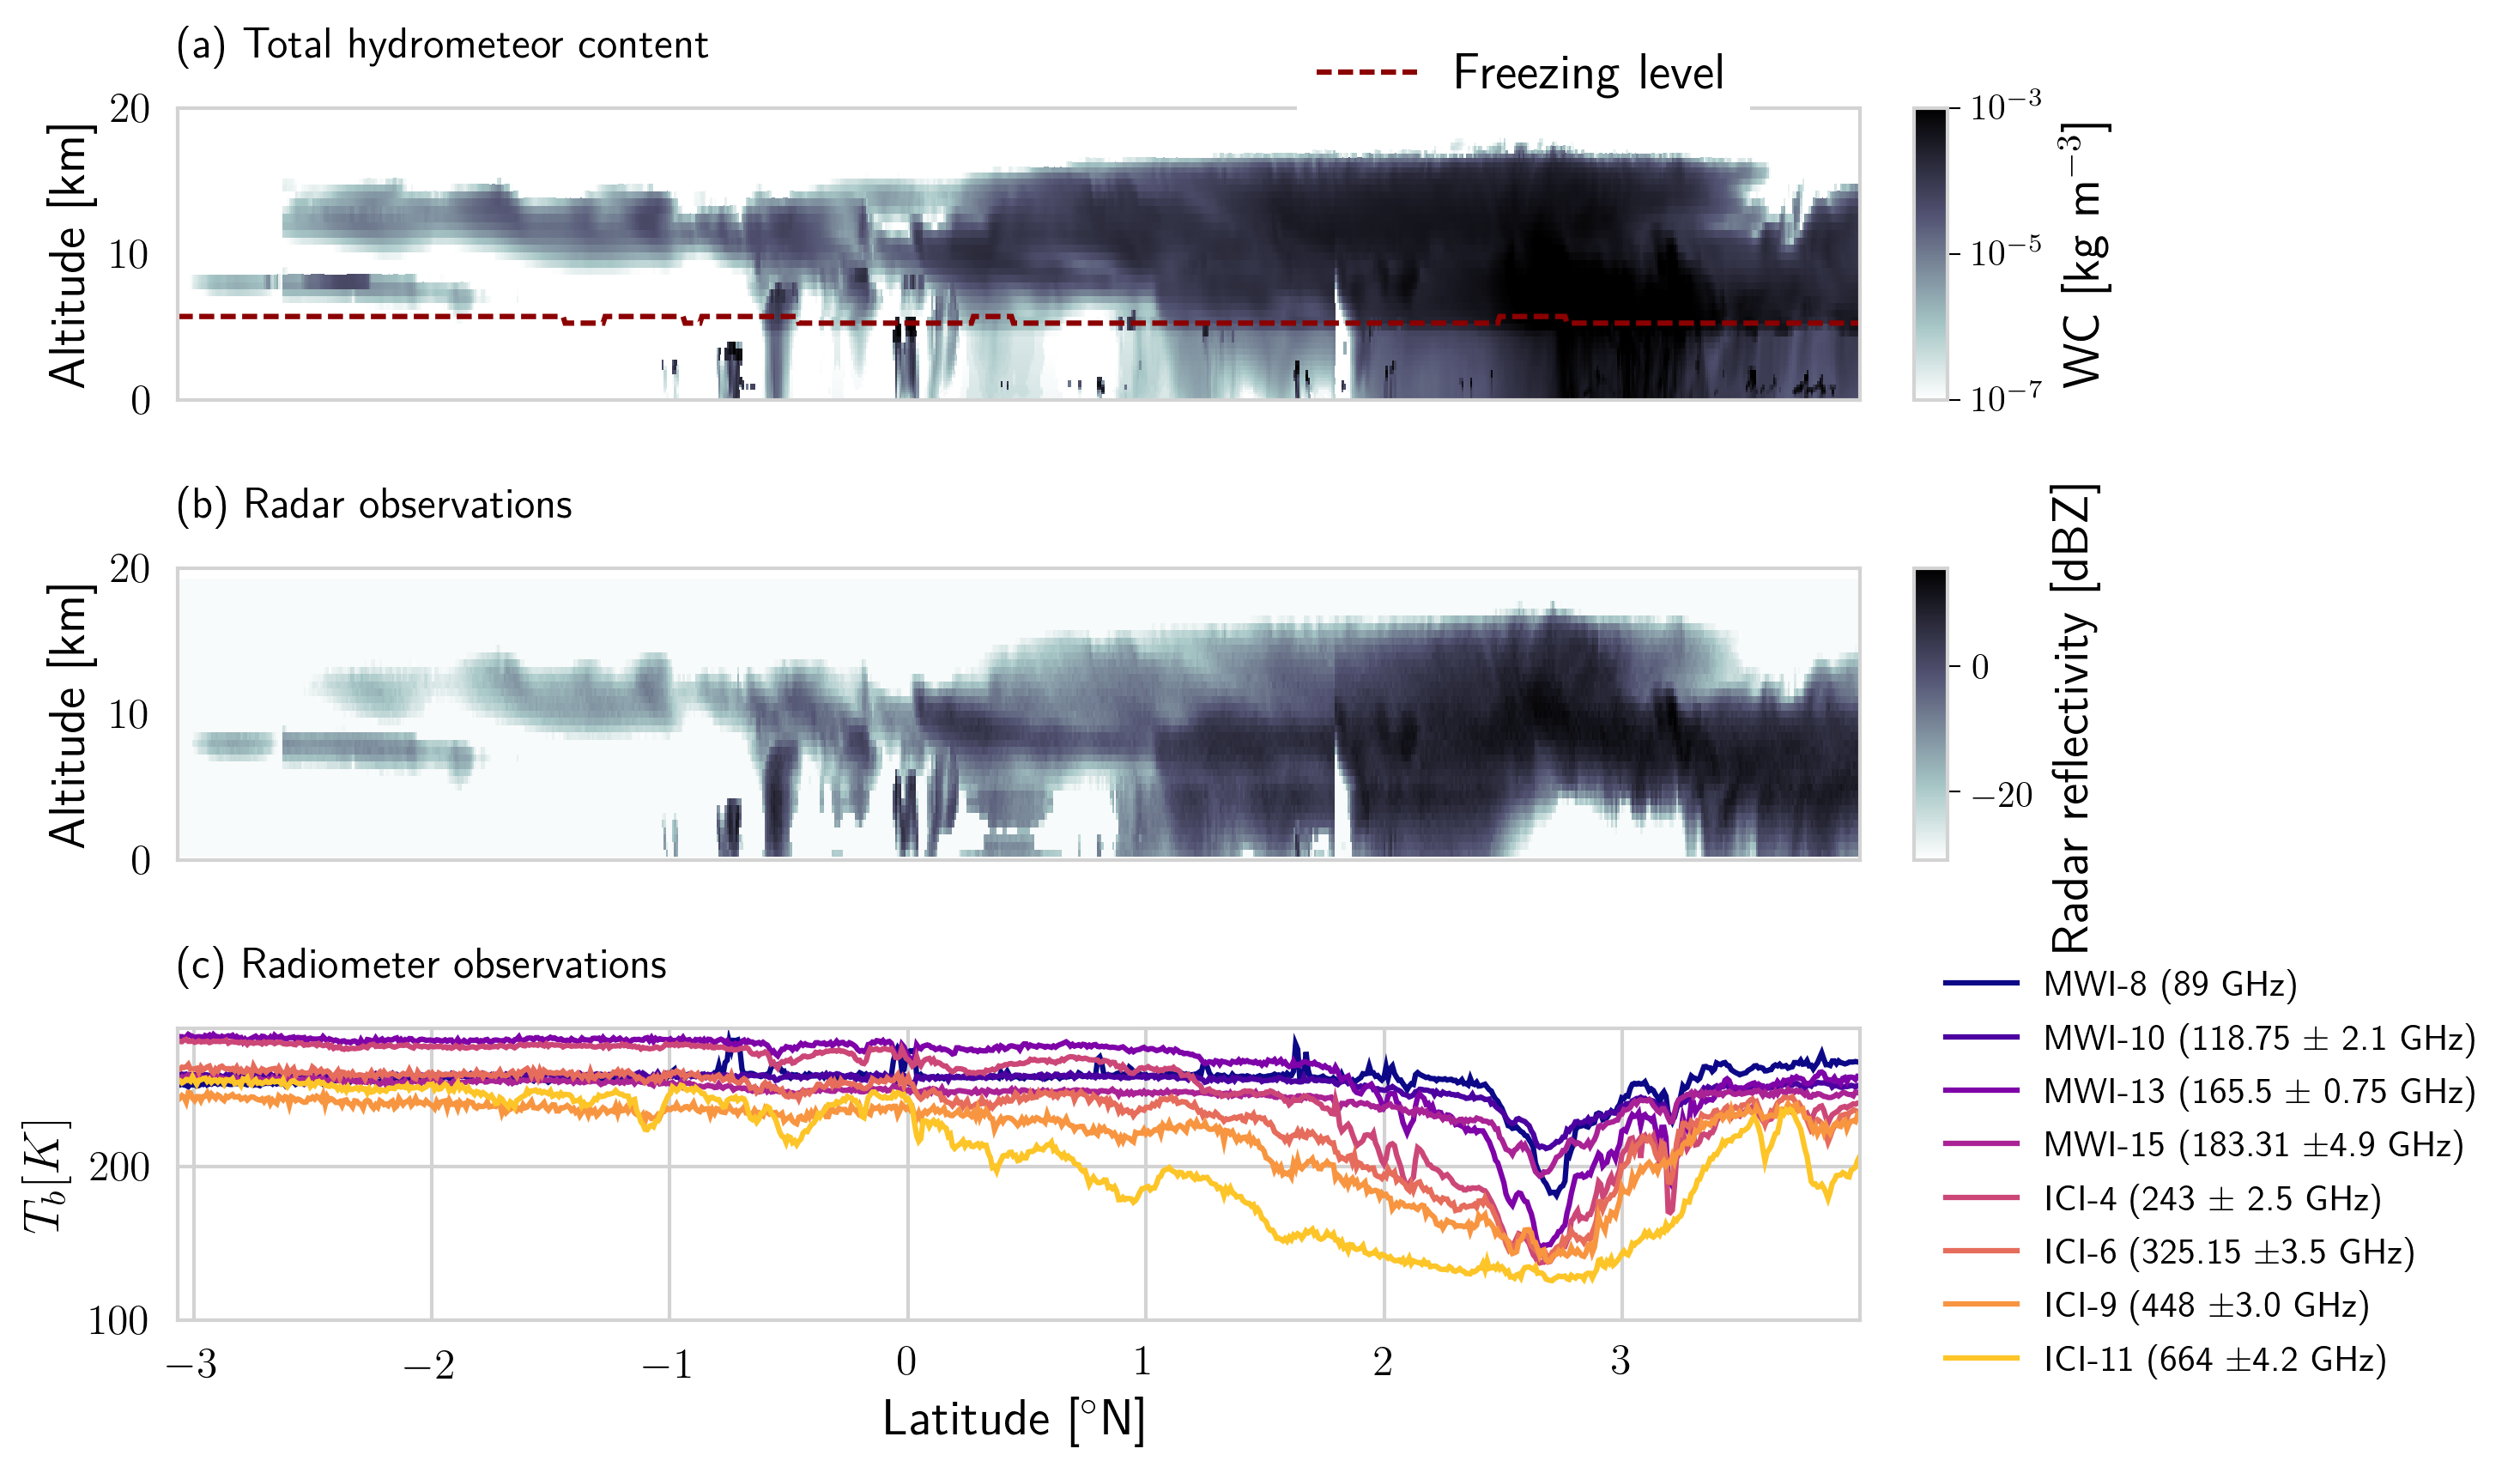
\includegraphics[width = 0.8\textwidth]{../plots/observations_a}
\caption{Total water content (WC) and simulated observations for the first test
  scene. Panel (a) displays the total water content in the scene, i.e. the sum
  of the water content of all hydrometeor species of the GEM model. Panel (b)
  shows the simulated radar reflectivities. Panel (c) displays the simulated
  brightness temperatures for a selection of channels of the MWI and ICI
  radiometers.}
\label{fig:observations_a}
\end{figure}

\subsubsection{Water content}

Results of the retrieved IWC obtained using the Large Plate Aggregate particle
mode for the first test scene are displayed in Fig.~\ref{fig:results_a}. The
reference IWC is defined here as the sum of the masses of the four frozen
hydrometeor species in the GEM model scenes.

The $\chi^2_y$ values of the three retrieval configurations, displayed in Panel
(a), give an indication of how well the retrievals are able to fit the
observations. For the radar-only retrieval, the values are much smaller than 1
for most parts of the scene, while for the passive-only and combined retrieval
they are around the expected value of 1. This indicates that the radar-only
retrieval overfits the observations, while the passive-only and combined
retrievals achieve the expected fit. The exception is the region around
$3^\circ\ N$, where the cloud is particularly thick and consists of a mix of
different hydrometeor types. Here, especially the passive-only retrieval has
problems fitting the observations.

In terms of IWP, all methods provide fairly good estimates of the reference
values with the combined retrieval consistently yielding the smallest deviations.
Larger differences between the methods are observed when comparing the retrieval
results in terms of IWC. While the vertical structure of the cloud is captured
only very roughly by the passive retrieval, it is better resolved by the
radar-only and the combined retrieval. On closer inspection, however, it becomes
evident that the radar-only retrieval deviates systematically from the reference
IWC in specific regions of the cloud, such as for example the upper part of the
cloud between $0^\circ N$ and $2^\circ N$. These deviations are corrected in the
results from the combined retrieval, although certain retrieval artifacts are
visible.

\begin{figure}
\centering
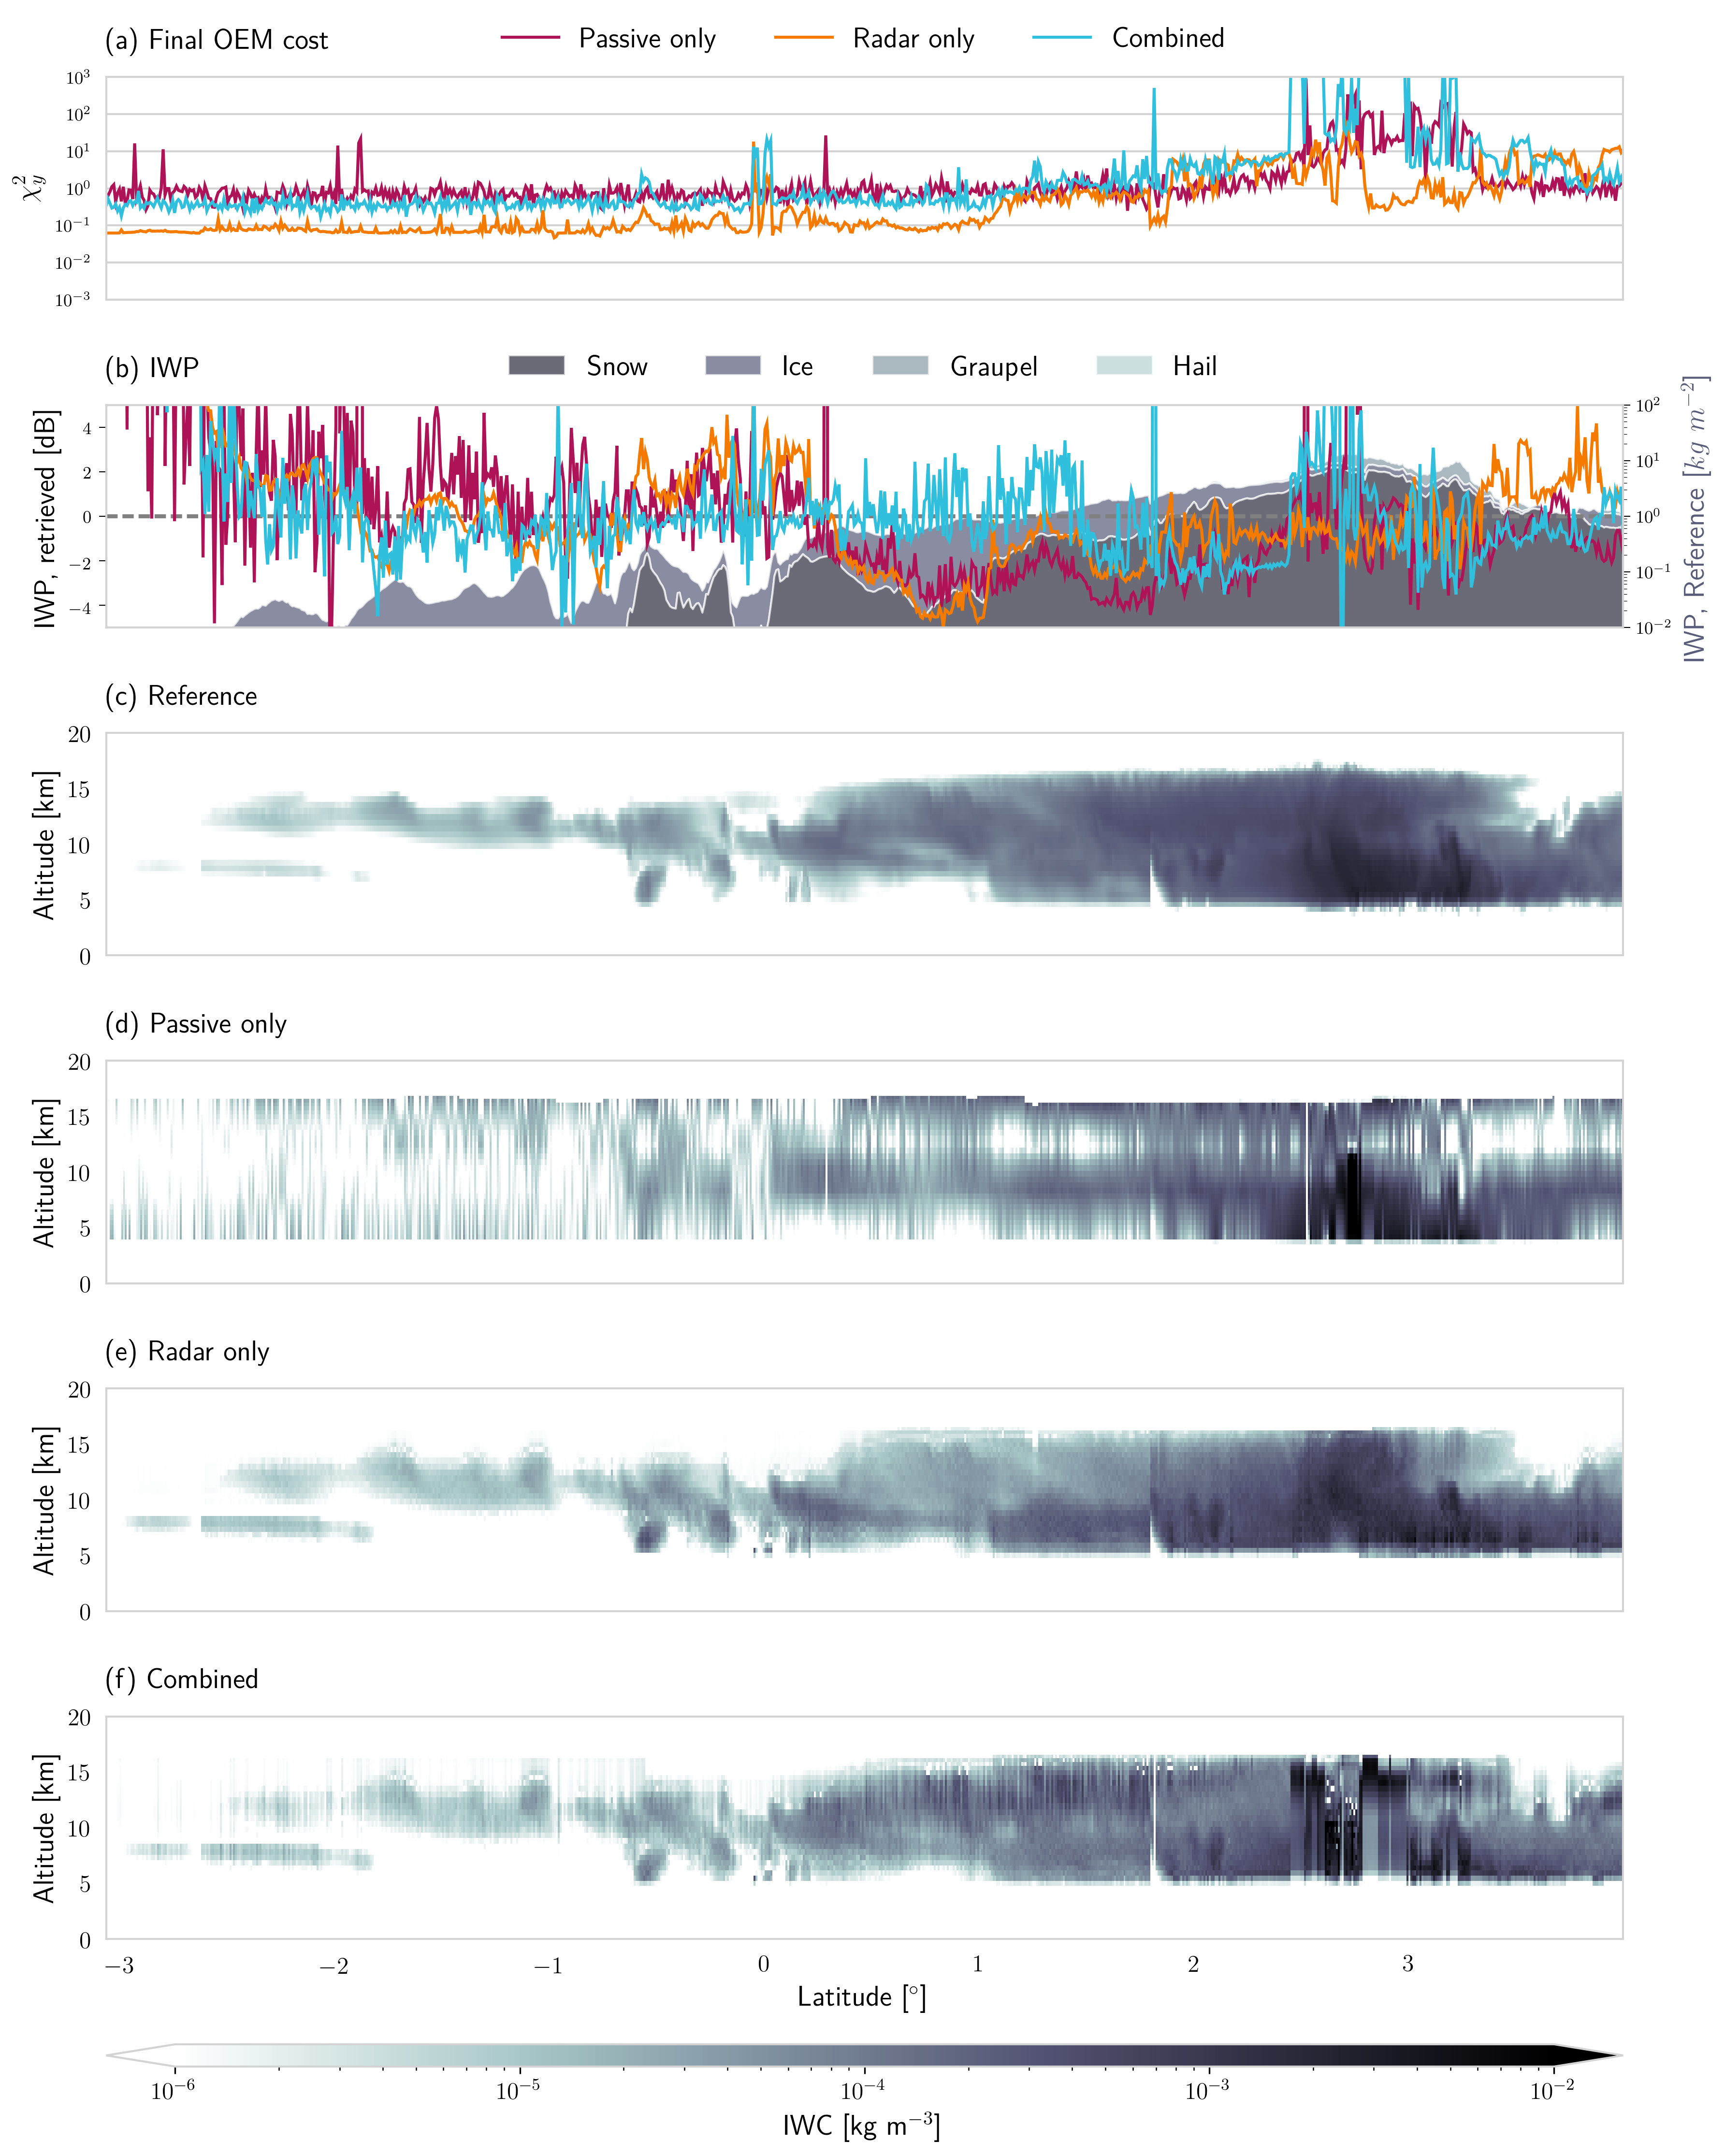
\includegraphics[width = 0.8\textwidth]{../plots/results_a_LargePlateAggregate}
\caption{Results of the ice hydrometeor retrieval for the first test scene using
  the Large Plage Aggregate particle shape. Panel (a) displays the value of the
  $\chi^2_y$ diagnostic normalized by the dimension of the measurement space of
  the corresponding retrieval. Panel (b) displays retrieved IWP in dB relative
  to the reference IWP. Reference IWP and the contributions from different
  hydrometeor classes are displayed by the filled areas in the background. Panel
  (c) shows the reference IWC from the model scene. Panel (d), (e) and (f)
  display the retrieval results for the passive-only, radar-only and combined
  retrieval, respectively.}
\label{fig:results_a}
\end{figure}

For a more quantitative assessment of the retrieval performance, retrieved water
content is plotted against the reference water content in
Fig.~\ref{fig:results_scatter_a}. In terms of precision, the passive-only
retrieval performs worst while both the radar-only and combined retrieval yield
much smaller spread in the retrieved values. This is not surprising considering
that the passive observations do not contain sufficient information on the
vertical distribution of IWC to yield accurate results at the resolution of the
model scenes. In terms of overall accuracy, i.e. systematic deviations from the
diagonal, no clear differences between the three configurations are visible.
However, the color-coding with respect to hydrometeor species reveals that the
radar-only retrieval is biased for specific hydrometeor classes. In the combined
and even the passive-only results, this effect is weaker and the clusters are
generally moved towards the diagonal. For graupel, all retrievals perform badly
but this is likely due to it being present only in the core of the convective
system where the signals from all sensors can be expected to be saturated.

Comparing the results for different particle models, a clear dependency is
evident in the passive-only and the combined results while the radar-only
retrieval is affected the least. For the combined and passive-only
retrieval, the effect is consistent across the methods, with the GEM Cloud Ice
and Large Column Aggregate yielding the largest deviations and the Large Plate
Aggregate yielding the most accurate results.

\begin{figure}
\centering 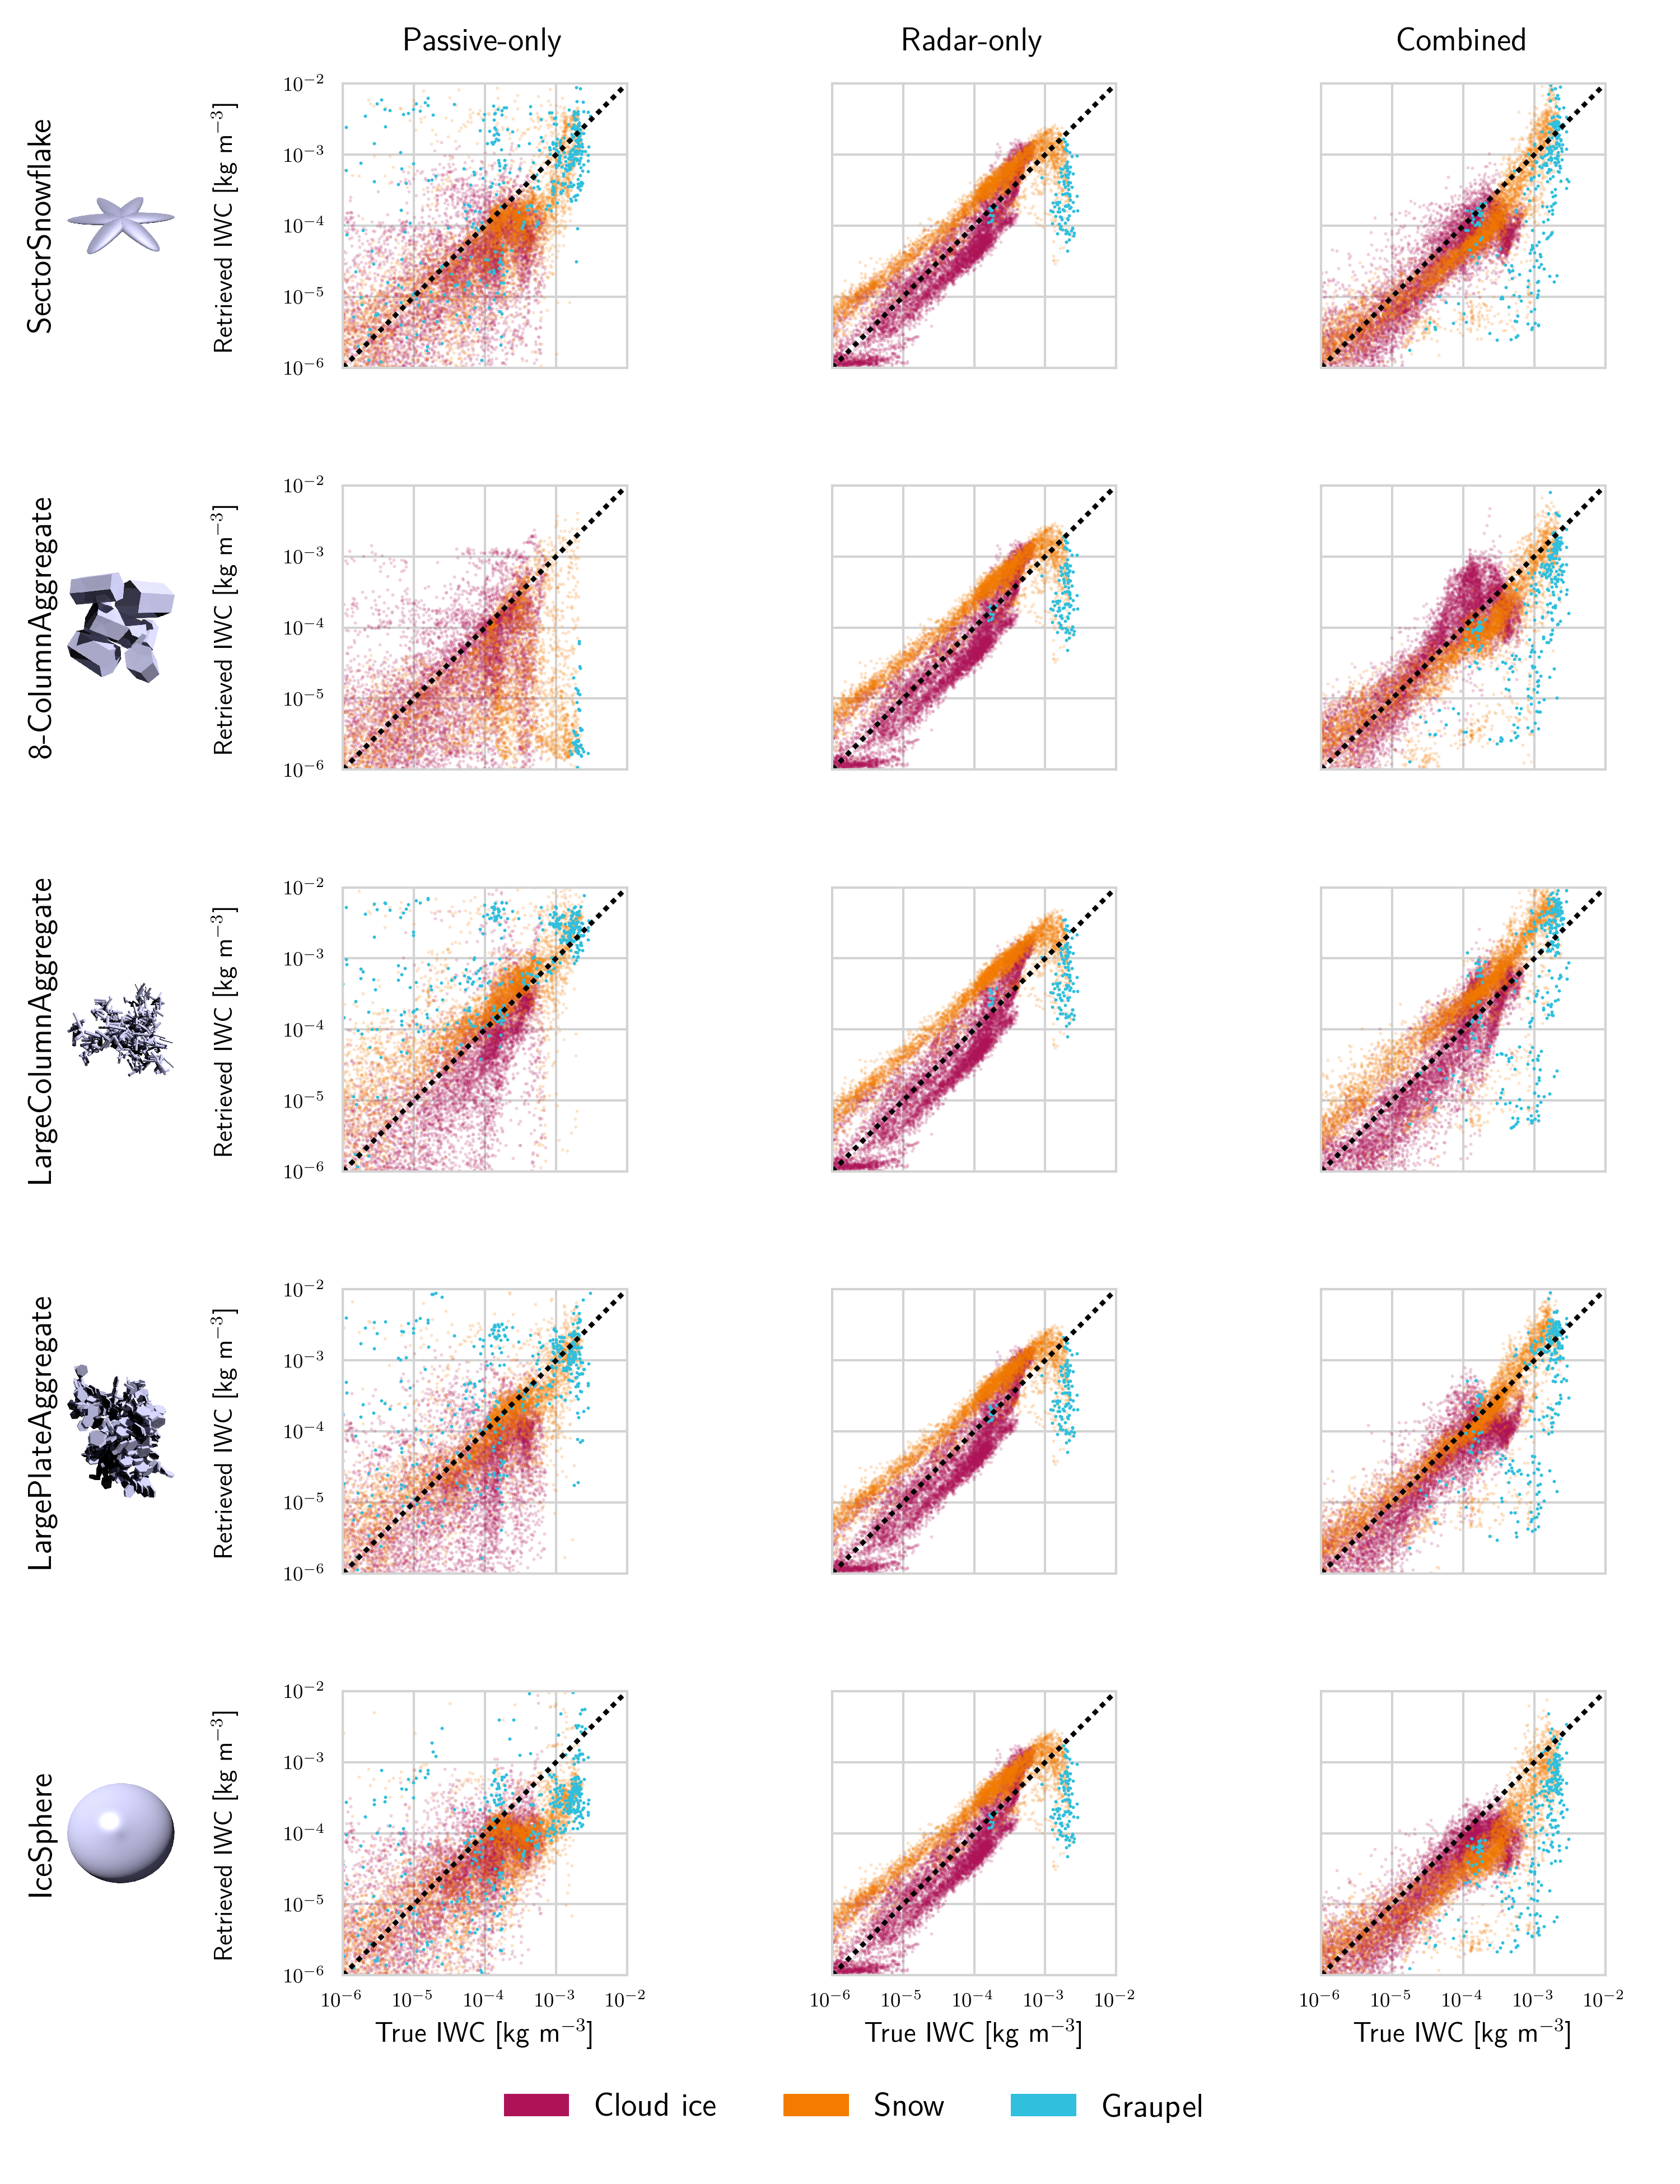
\includegraphics[width = 0.75\textwidth]{../plots/results_scatter_a}
\caption{Retrieved IWC plotted against reference IWC for the tested retrieval
  configurations. Each row shows the retrieval results for the particle shape
  shown in the first panel. The following panels show the retrieval results for
  the passive-only (first column), the radar-only (second column) and the
  combined retrieval (third column). Markers are colored according to the
  prevailing hydrometeor type at the corresponding grid point in the test
  scene. Due to their sparsity, markers corresponding to graupel are drawn at
  twice the size of the other markers.}
\label{fig:results_scatter_a}
\end{figure}

To summarize retrieval performance for all tested retrieval methods and particle
shapes, the distributions of the logarithmic error
\begin{align}
  \text{E}_{\text{log}_{10}} &= \log_\text{10} \left
  (\frac{x_\text{retrieved}}{x_\text{reference}} \right )
\end{align}
for the retrieved IWC and IWP are displayed in Fig.~\ref{fig:boxes}. In addition
to the two-moment version of the radar-only retrieval, this figure also displays
results of the single-moment version of the retrieval, which was actually found
to yield better IWC retrievals for one of the scenes.

The error for IWC has been computed considering only grid points where either
reference or retrieved IWC is larger than $10^{-6}\ \unit{kg\ m^{-3}}$. Similar
to the results presented above, the combined retrieval yields the smallest
retrieval errors for suitable choices of the particle model. Although the
two-moment radar-only retrieval performs similar to the combined retrieval in
terms of precision, it yields significant systematic errors for the second
scene. The reason for this can be understood considering the cloud composition
displayed in Fig.~\ref{fig:overview}. Since the clouds in the second test scene
consist mostly of snow, the bias of the radar-only retrieval with respect to
this specific hydrometeor species (c.f. Fig.~\ref{fig:results_scatter_a} and
also Fig.~\ref{fig:results_scatter_b}) leads to the large observed systematic
errors for the second scene. The single-moment radar-only retrieval does not
produce the same large systematic errors for the second scene, but instead
produces systematic errors for the first scene. The passive-only retrieval
yields the largest errors in terms of retrieved IWC due its low vertical
resolution.

In terms of IWP, however, the errors of the passive-only retrieval are decreased
making the retrieval comparable to the other methods. For the radar-only
and combined retrievals, the precision is generally increased but the systematic
deviations observed for IWC persist. This leads, particularly for the second
test scene, to significant systematic errors in the IWP retrieved by the
two-moment radar-only retrieval.

Also in these results, a strong dependence on the applied particle model is
observed for the passive-only and combined retrievals. The errors are
particularly large for the GEM Cloud Ice and the Large Column Aggregate. For the
radar-only retrieval, the particle shape has less impact on the retrieval
performance and does not affect the large systematic errors observed for the
second test scene.

\begin{figure}[!h]
\centering 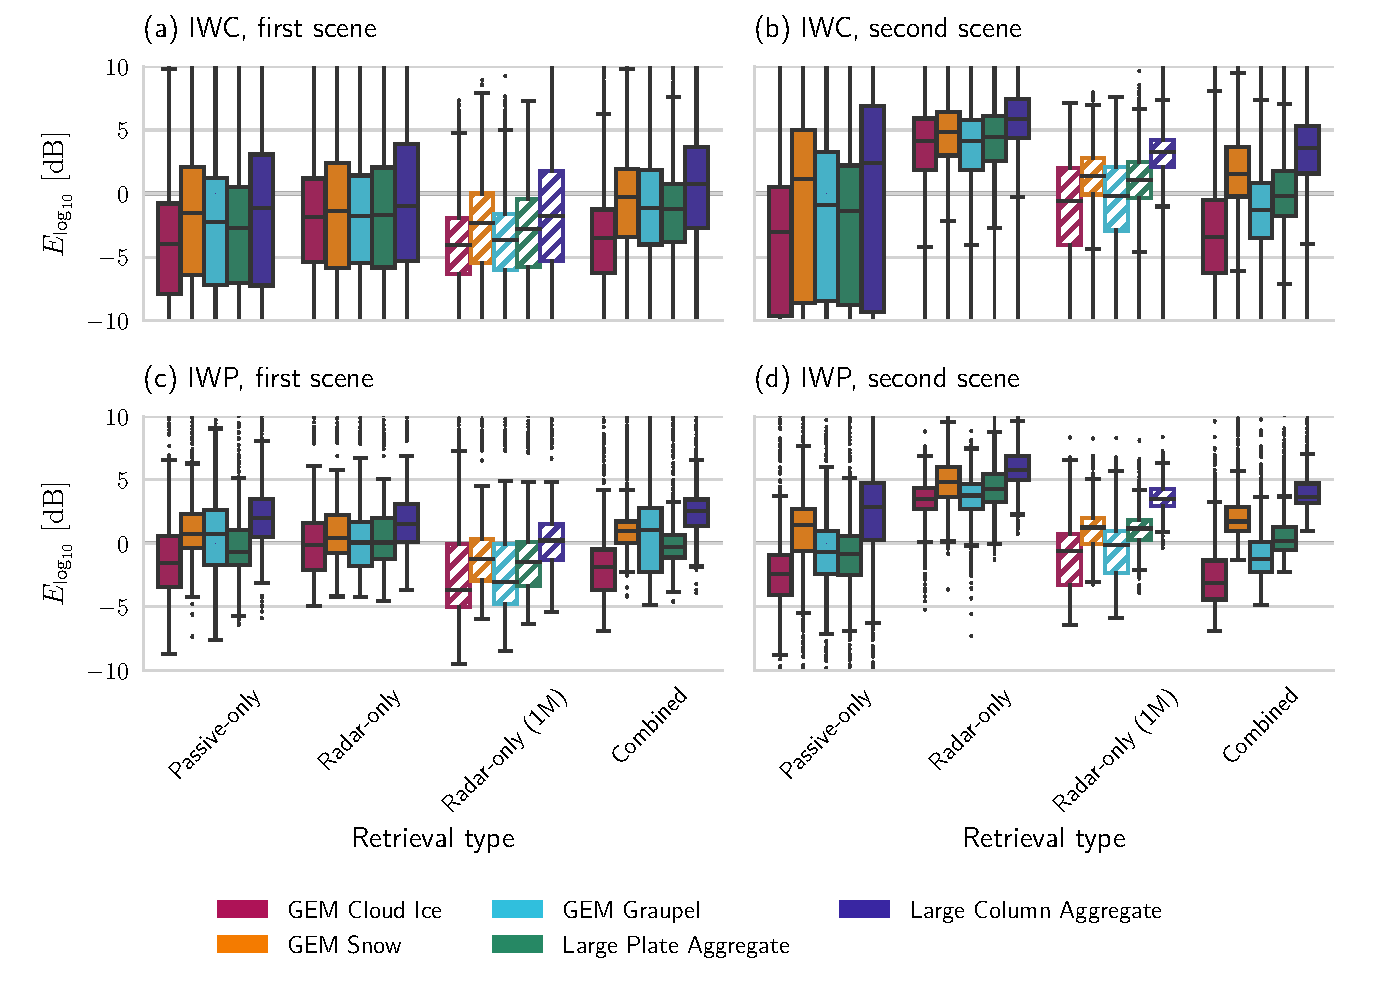
\includegraphics[width = 0.8\textwidth]{../plots/results_box}
\caption{Distributions of the logarithmic retrieval error in IWC and IWP for all
  tested retrieval methods and particle shapes displayed as box plots. Colored
  boxes display the interquartile range (IQR) while whiskers show the full range of
  all points not considered outliers. Points whose distance to the IQR is larger
  than 1.5 times the width of the IQR are considered outliers and drawn as
  markers. Two results are shown for the radar-only retrieval, one for the
  standard version retrieving both PSD moments (solid boxes) and one for the
  single-moment (1M) version (diagonal hatches).}
\label{fig:boxes}
\end{figure}

\subsubsection{Particle number concentrations}

Particle number concentrations of frozen hydrometeors have been derived from the
retrieved $N_0^*$ and $D_m$ parameters by computing the zeroth moment of the
corresponding PSD. The resulting particle number concentration fields are displayed
together with the reference field in Fig.~\ref{fig:results_nd_a}. To simplify
the comparison, number concentrations are displayed only where the corresponding
reference or retrieved IWC is larger than $10^{-6}\ \unit{kg\ m^{-3}}$.

Comparing the passive-only and the radar-only retrieval to the reference fields
shows that both methods have little to no skill in predicting number 
concentrations. Although the passive-only retrieval partly captures the gradient
between very high concentrations at the top of the cloud and the low
concentrations at the bottom, it is not at all resolved in the radar-only
retrieval.

In contrast to this, the combined retrieval manages to reproduce this gradient
in most parts of the scene. The strongest deviations of the combined results
from the reference field are observed between $2\ \unit{^\circ \ N}$ and
$3\unit{^\circ \ N}$ latitude. Here, the results strongly underestimate the true
number concentrations. Comparison with the cloud composition displayed in Panel
(a) of Fig.~\ref{fig:overview} shows that this region contains large amounts of
both cloud ice and snow. The retrieval uses only a single hydrometeor species to
represent ice in the atmosphere and is therefore not able to represent such
heterogeneous conditions. Since snow will have a stronger impact on the
observations, the retrieval in these regions will likely tend to represent snow
rather than ice, which leads to the low retrieved number concentrations.

\begin{figure}
\centering
\includegraphics[width = 0.7\textwidth]{../plots/results_nd_a_LargePlateAggregate}
\caption{Reference and retrieved particle number concentrations of frozen
  hydrometeors for the first test scene obtained with the LargePlateAggregate
  particle model. Panel (a) displays the reference water content from the
  model scene. Panel (b), (c) and (d) display the retrieval results for the
  passive-only, radar-only and combined retrieval. Only values for which the
  corresponding reference or retrieved IWC was larger than
  $10^{-6}\ \unit{kg\ m^{-3}}$ are shown here.}
\label{fig:results_nd_a}
\end{figure}

Fig.~\ref{fig:results_nd_scatter_a} displays scatter plots of the reference and
retrieved particle number concentrations for all three methods and two particle
models from the first test scene. Markers in the plot are color coded according
to their homogeneity in the reference scene, here defined as the ratio of the
maximum water content of any of the frozen hydrometeor species and the total
water content. These results confirm that the passive-only retrieval possesses
some sensitivity to the particle number concentrations since the cluster at low
concentrations corresponding to snow is placed correctly on the diagonal, which
is not the case for the radar-only retrieval. The radar-only retrieval does not
exhibit any retrieval skill, hardly reproducing any of the variation of the
reference values. Contrary to this, the combined retrieval moves both clusters,
the one corresponding to snow and the one at high number concentrations
corresponding to cloud ice, towards the diagonal. This indicates that it is
capable of distinguishing the microphysical properties of cloud ice and snow.
Furthermore, the color coding shows that the strongest deviations between
retrieved and reference number concentrations occur for grid points where the
cloud composition is heterogeneous.

The general effect of particle shape on the retrieval results is similar to what
has been observed for IWC, which is why only results for two particle shapes are
shown. For the passive-only and combined retrieval, the GEM Cloud Ice and Large
Column Aggregate models yield the worst retrieval results, while the Large Plate
Aggregate performs best. For the radar-only retrieval no noticeable differences
are observed between different particle models.

\begin{figure}
\centering
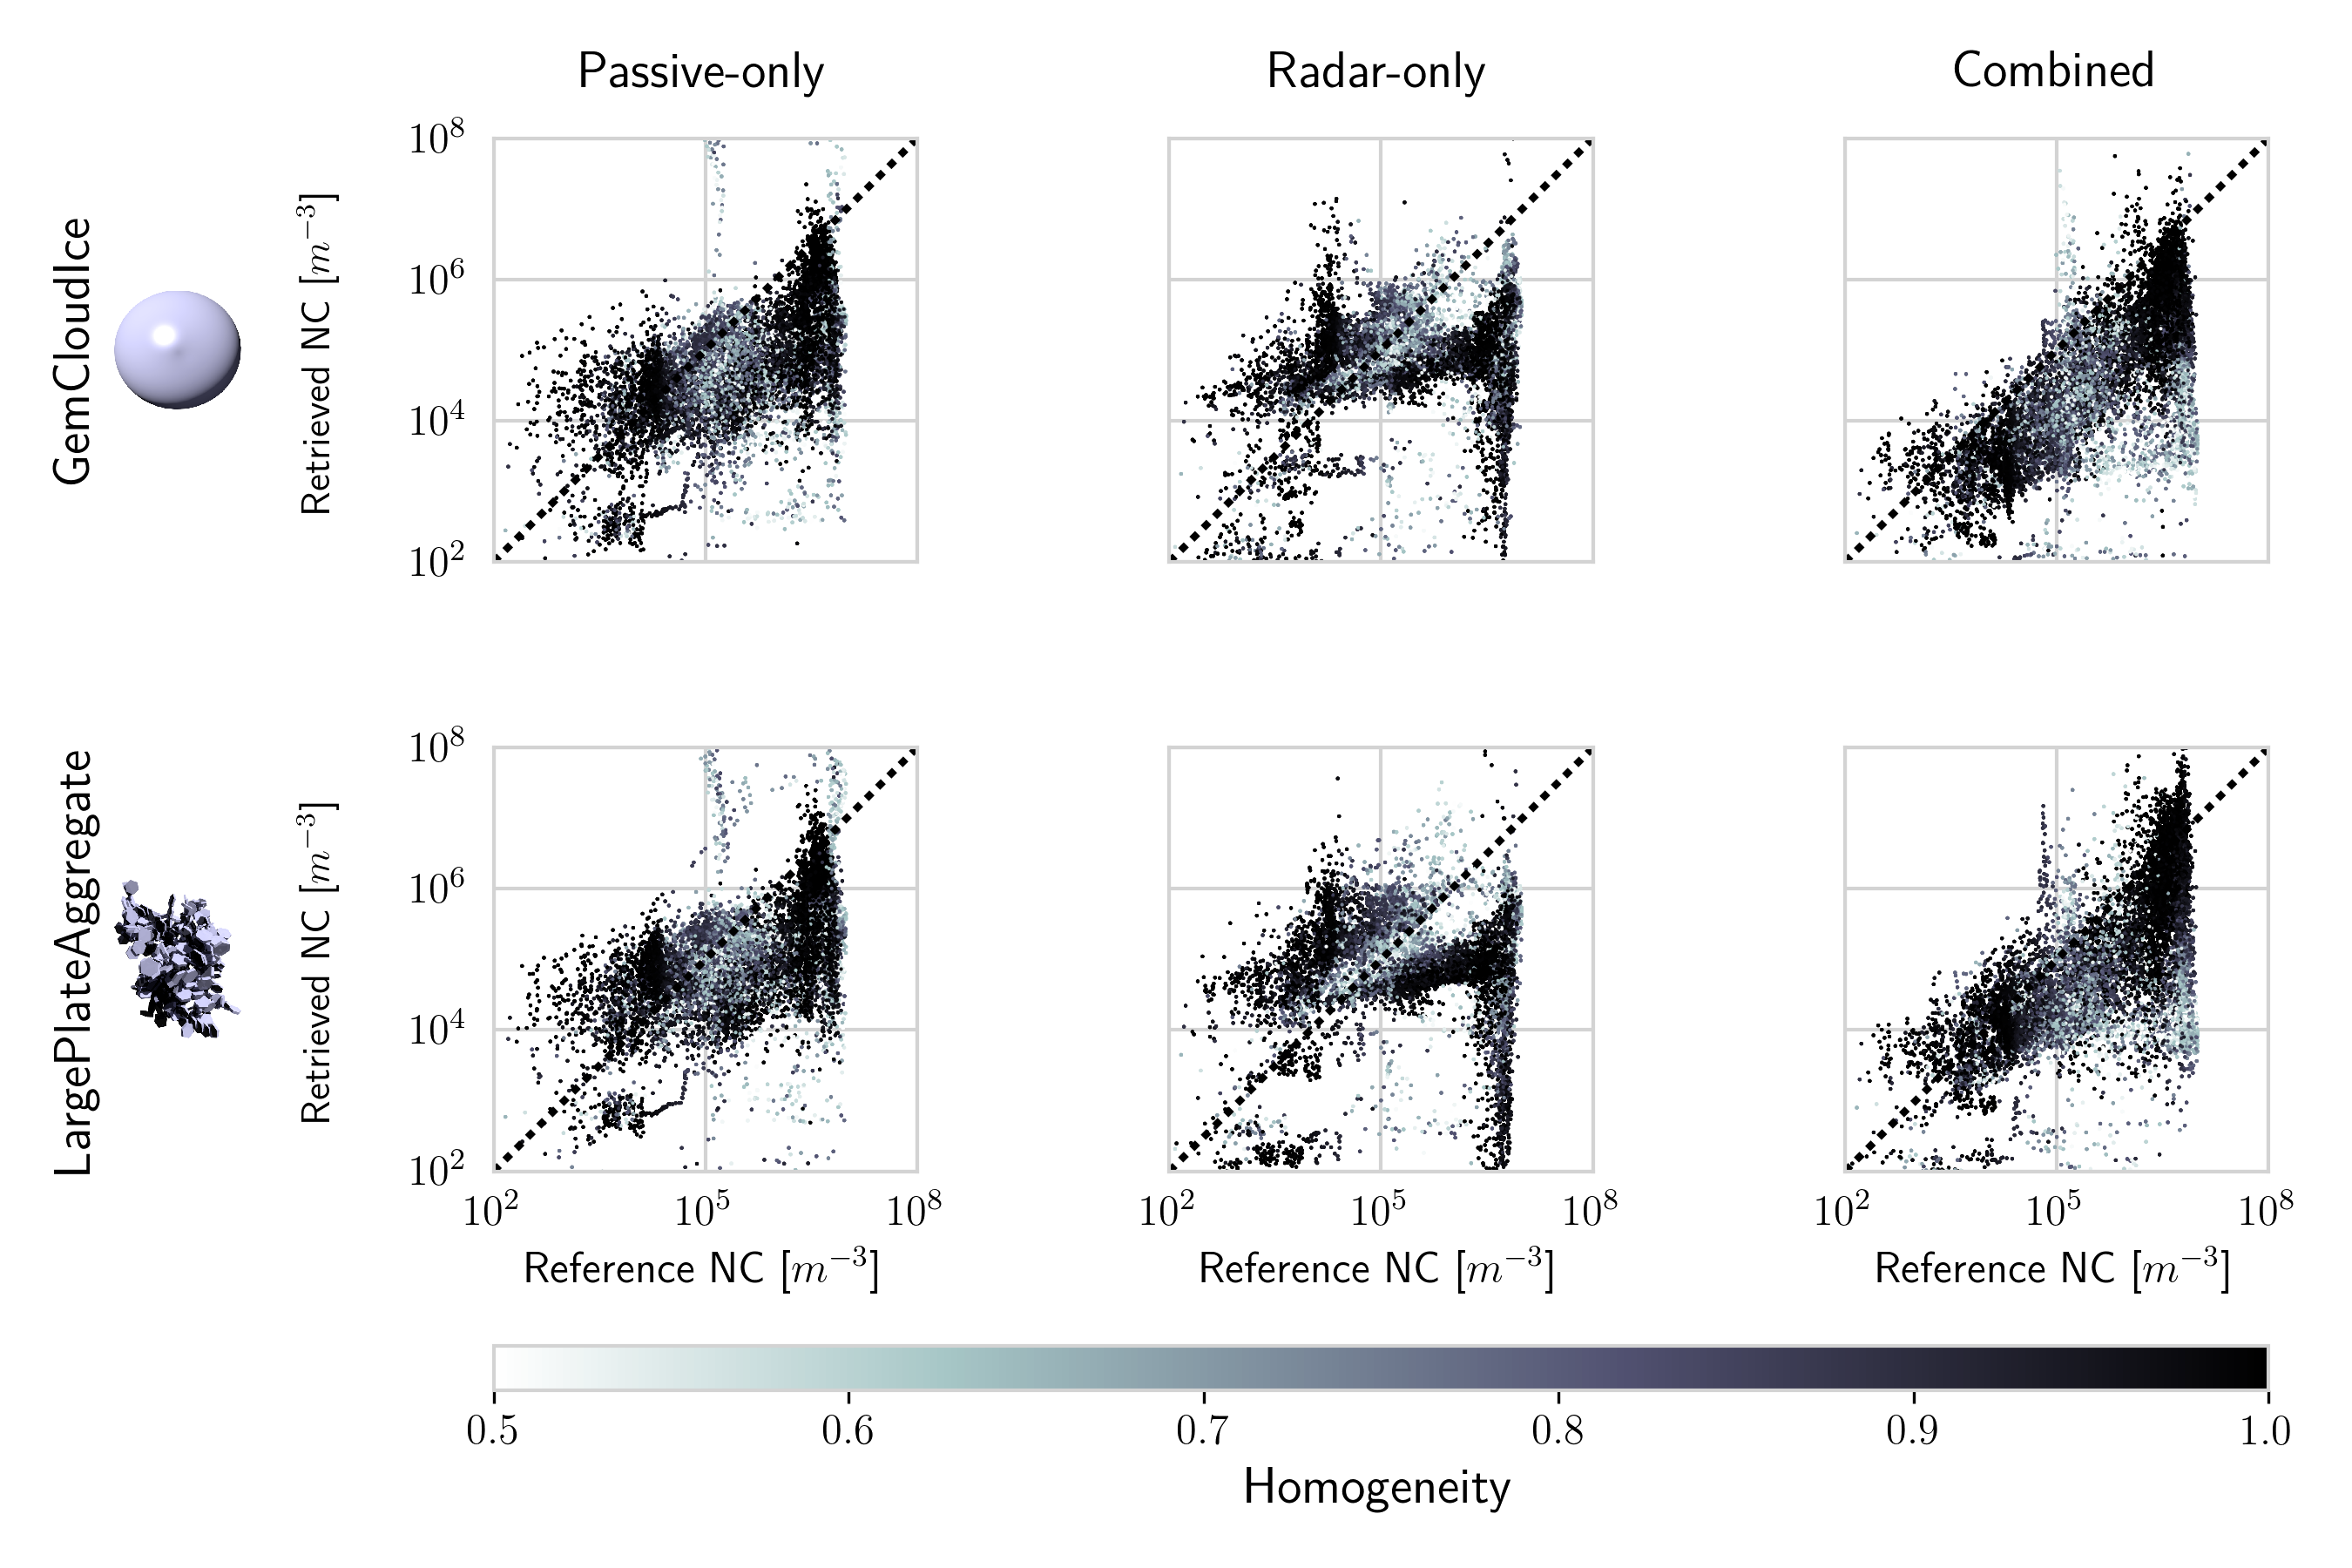
\includegraphics[width = 0.7\textwidth]{../plots/results_nd_scatter_a}
\caption{Scatter plots of the retrieved particle number concentrations at grid points
  with reference IWC larger than $10^{-5}\ \unit{kg\ m^{-3}}$. Rows show
  the results for the different particle models used in the retrieval while
  columns display  results for  different retrieval methods. The marker
  color encodes the homogeneity of the corresponding ice mass, which is computed
  as the ratio of the maximum water content of any of the frozen hydrometeor
  species and total IWC.}
\label{fig:results_nd_scatter_a}
\end{figure}

\subsubsection{Information content}

To quantify the information content of the single-instrument and the combined
observations, the degrees of freedom for signal (DFS) have been computed
following \cite{rodgers00} by calculating the trace of the averaging kernel
matrix
\begin{align}
  \mathbf{A} &= (\mathbf{K}^T \mathbf{S}_e^{-1} \mathbf{K} +
  \mathbf{S}_a^{-1})^{-1} \mathbf{K}^T \mathbf{S}_e^{-1} \mathbf{K},
\end{align}
where $\mathbf{K} = \frac{d\mathbf{F}(\mathbf{x})}{d\mathbf{x}}$ is the Jacobian
of the forward model. The information content and its decomposition into
contributions from different retrieval quantities are displayed in
Fig.~\ref{fig:dfs}.

With respect to ice, the passive-only retrieval yields the lowest information
content. For the radar-only retrieval the information content is significantly
higher, on the order of 20 degrees of freedom, but the major part of it is
attributed to the $D_m$ parameter. For the combined retrieval, the total
information content on ice hydrometeors is increased compared to the radar-only
retrieval in regions where the passive-only retrieval provides information on
frozen hydrometeors. In addition to that, a clear shift of information content
from $D_m$ to $N_0^*$ can be observed over both scenes.

The information content for rain is much smaller but in relative terms the
general behavior is the same as for ice. For RH, no difference is observed for
the information content provided by the passive-only and combined retrievals.
For LCWC, the information content of the combined observations is increased
slightly but remains limited to a few degrees of freedom.

\begin{figure}
\centering
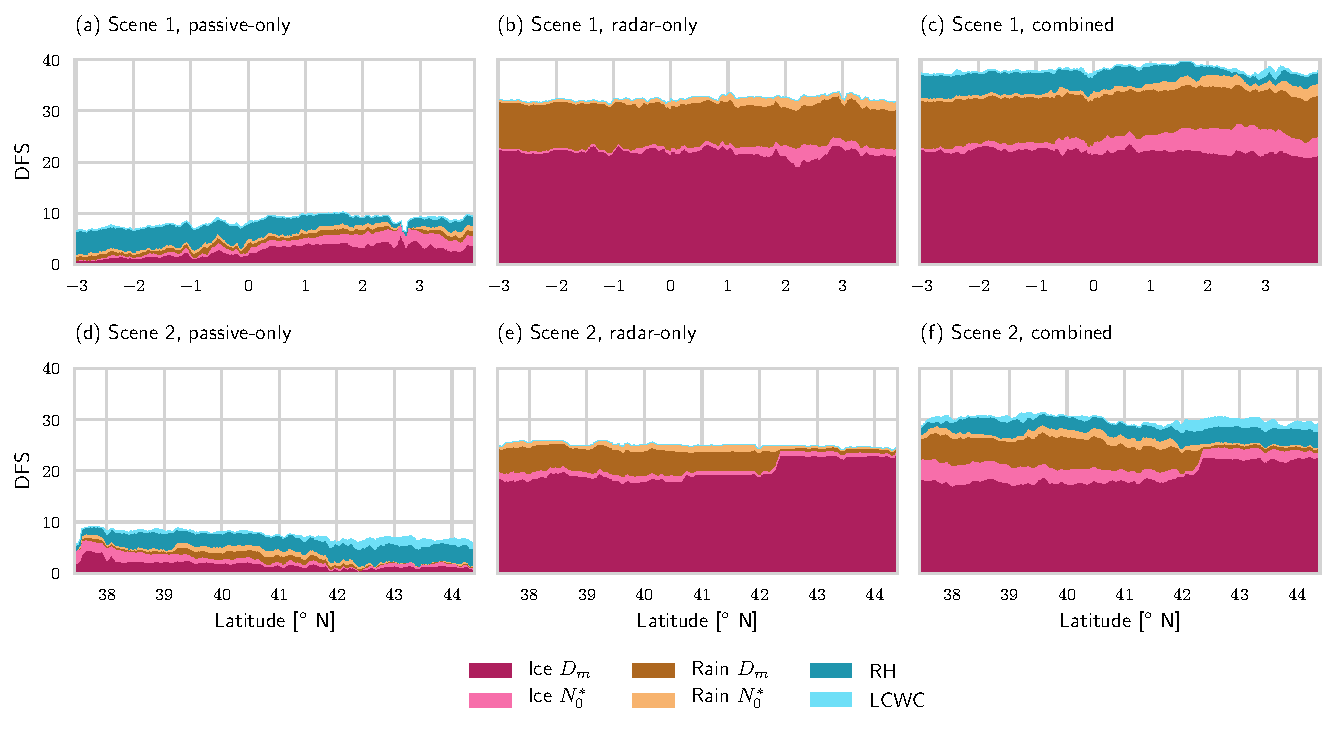
\includegraphics[width = 1.0\textwidth]{../plots/dfs}
\caption{Degrees of freedom for signal for all retrieval configurations and both
  test scenes obtained with the Large Plate Aggregate model. The colored areas
  in each plot represent the contribution to the cumulative degrees of freedom
  from each retrieval quantity. Results for the first and second test scene
  are displayed in the first and second row, respectively. The first, second
  and third panel in each row show the results for the passive-only, radar-only
  and the combined retrieval.}
\label{fig:dfs}
\end{figure}

\subsubsection{Impact of assumed ice particle shape}

The impact of the assumed ice particle shape on the retrieval results raises the
question whether it also affects the quality of the fit to the observations. To
investigate this, the residuals for the radar observations and three ICI
channels are displayed in Fig.~\ref{fig:misfit}. Each test scene contains a
region where the retrieval does not fit the observations well and where
substantial deviations between the fitted and true observations are observed. It
is also in these regions, where the fits obtained with different particle models
differ. These are both regions where the cloud is very thick and both the radar
and passive observations are likely saturated. Since these are difficult regions
for the retrieval it remains unclear whether these differences can be related
directly to the assumed particle shape. In contrast to this, the retrieval fits
the observations well in the remaining parts of the scene. The exception is the
GEM Graupel particle, for which quite significant misfits are observed in the
first test scene between $0\ \unit{^{\circ}\ N}$ and $1\ \unit{^{\circ}\ N}$
latitude.

\begin{figure}[!h]
\centering
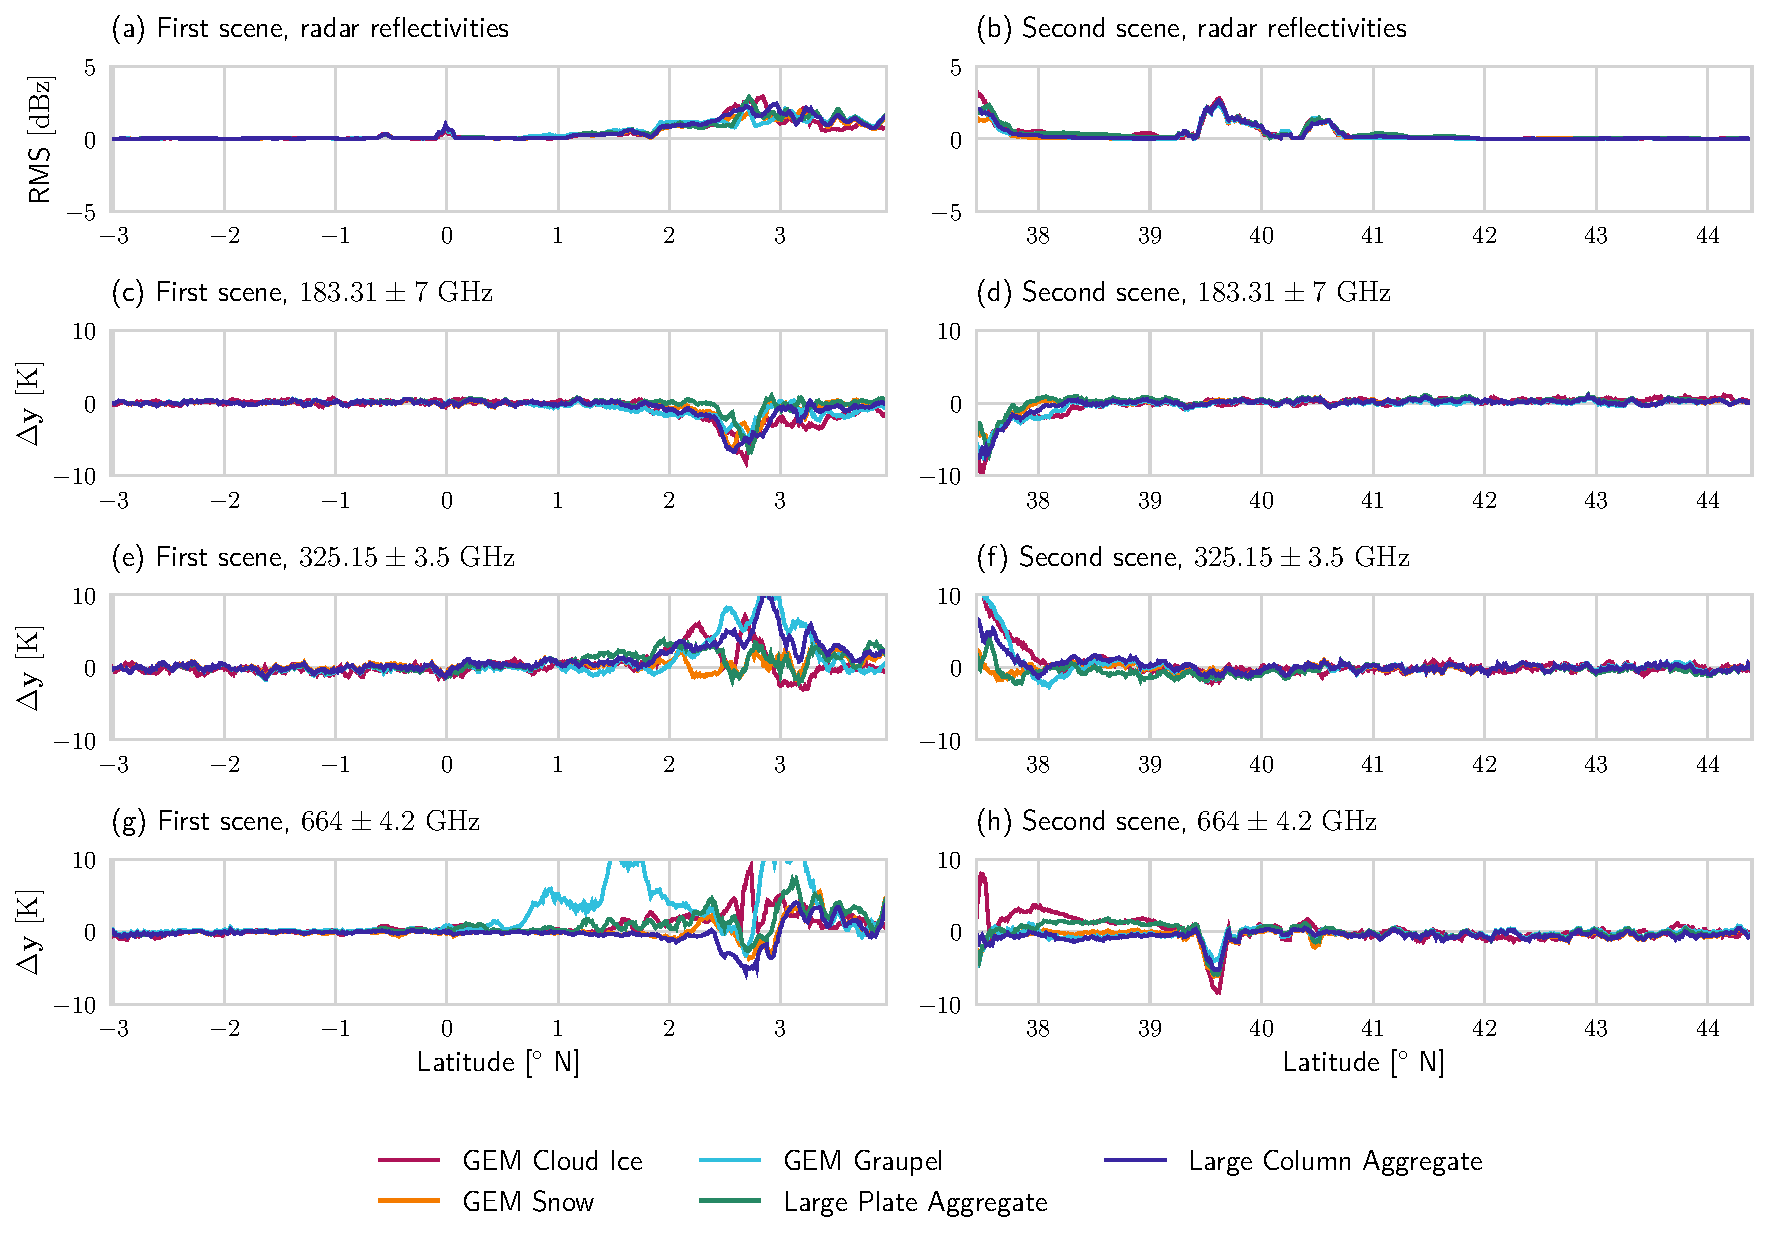
\includegraphics[width = 0.8\textwidth]{../plots/misfits}
\caption{Residuals of the fitted observations. First row of panels shows the
  profile root mean squared error (RMS) between fitted ($\hat{\mathbf{y}}$) and
  true ($\mathbf{y}$) radar observations for the two test scenes. Rows 2, 3 and
  4 show the residual $\Delta \mathbf{y} = \hat{\mathbf{y}} - \mathbf{y}$ for a
  selection of ICI channels.}
\label{fig:misfit}
\end{figure}

\subsubsection{Humidity and cloud water}

The developed passive and combined retrieval algorithms also retrieve profiles
of RH and LCWC. For RH, both retrievals demonstrate sensitivity but no
improvement was observed in the results of the combined retrieval compared to
the passive-only retrieval.

Results of the LCWC retrieval are shown in Fig.~\ref{fig:results_cw_b}. For the
retrieved LCWC, the combined retrieval yields slightly improved results compared
to the passive-only retrieval. The improvements are observed mostly in the
retrieved liquid cloud water path (LCWP) in the northern part of the scene. It
should be noted that the cloud in this part is a mixed-phase cloud and that both
retrievals successfully retrieve IWC and LCWC. At the center of the scene both
retrievals fail to retrieve the LCWC. The reason for this is that in these
regions rain is present, whose signal likely swamps any signal from the liquid
cloud droplets.

\begin{figure}
\centering
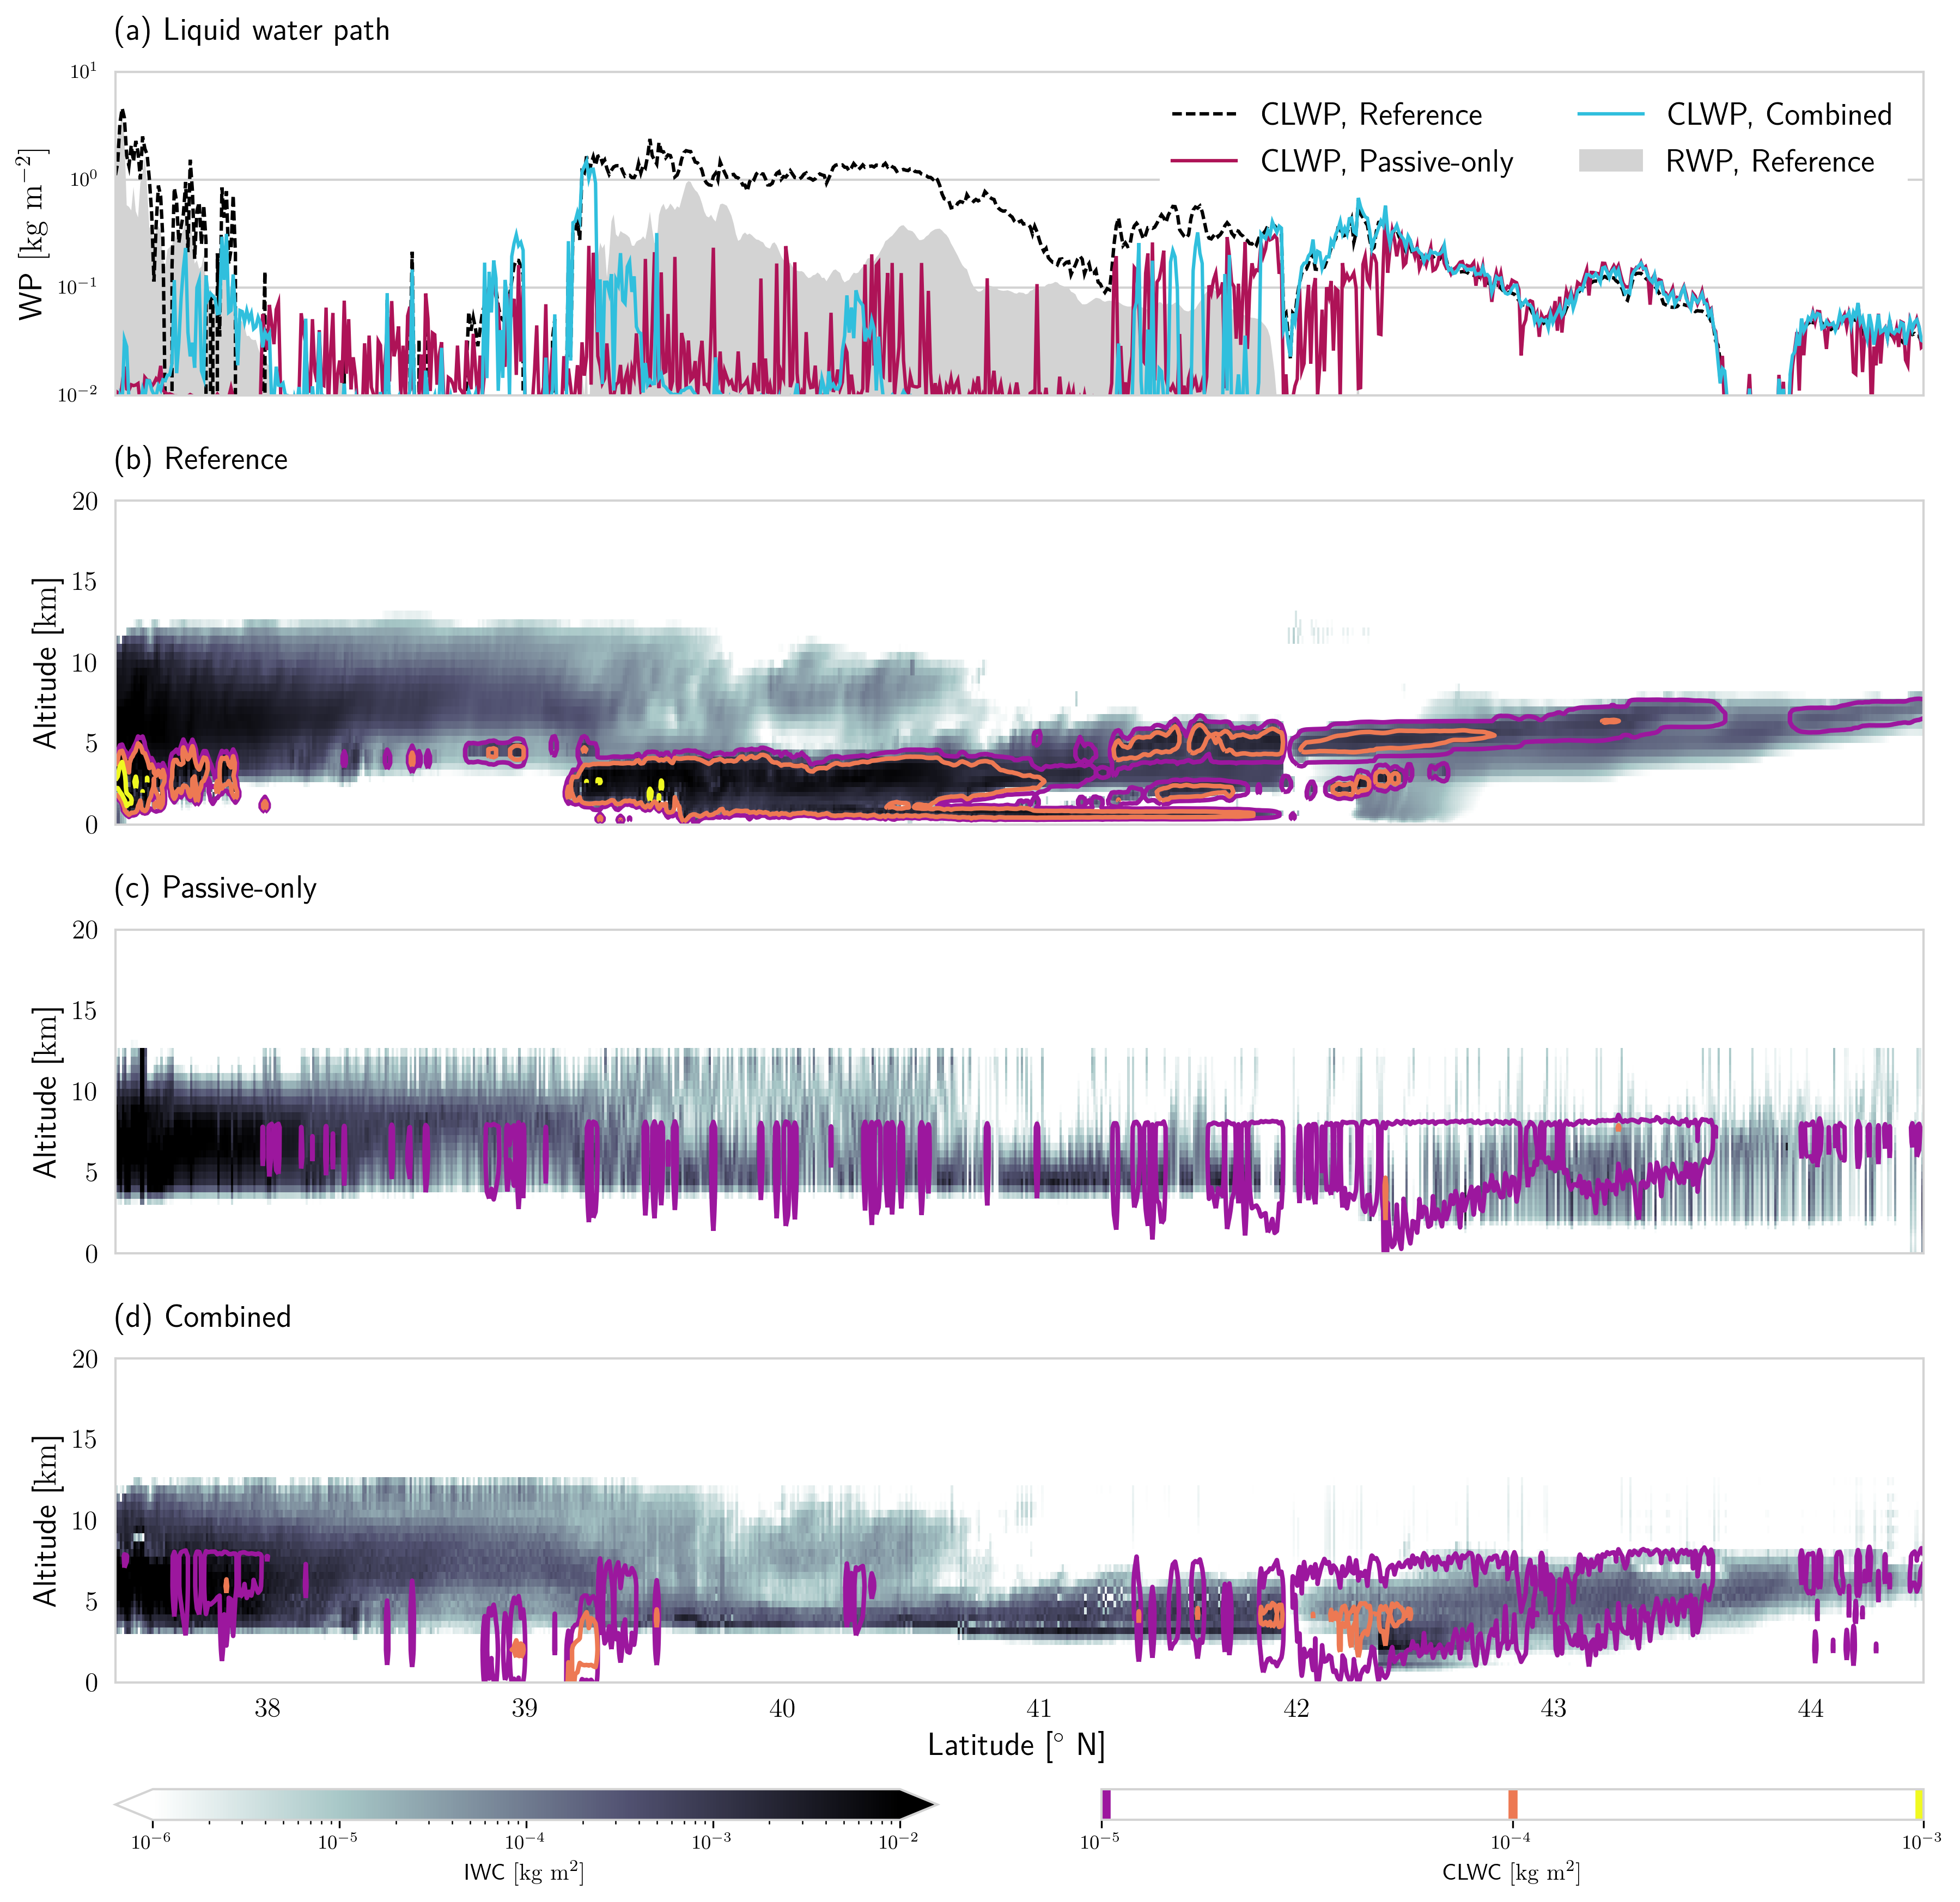
\includegraphics[width = \textwidth]{../plots/results_cw_b_LargePlateAggregate}
\caption{Reference and retrieved CLWC and IWC. Panel (a) shows the reference and
  retrieved LWP for each profile. Panel (b) displays reference LWC contours
  drawn on top of the total hydrometeor content. Retrieval results for
  passive-only and combined retrieval are given in Panel (c) and (d).}
\label{fig:results_cw_b}
\end{figure}


\section{Discussion}
\label{sec:discussion}

The principal aim of this study was to investigate the synergies between radar
and passive sub-millimeter observations for the retrieval of frozen
hydrometeors. To this end, a simplified numerical experiment has been presented,
which demonstrates the existence of complementary information in the radar and
passive microwave observations. Furthermore, a combined retrieval algorithm has
been developed to demonstrate the feasibility of the synergistic retrieval and
further explore their potential as well as current limitations.

The novelty of this work for lies, in part, in the application of ICI's
sub-millimeter channels, which sets it apart from the combined retrievals
developed for the TRMM and GPM missions. Moreover, the development of a fully
consistent variational retrieval in which all retrieval quantities are retrieved
simultaneously using observations from all sensors development is also novel.
This allows comparison of the synergistic retrieval to equivalent radar-only and
passive-only configurations and therefore a direct analysis of the synergies
between the active and passive observations.

\subsection{Fundamental synergies}

The experiment presented in the first part of this study aimed to illustrate the
fundamental synergies of active and passive microwave observations. It compared
the cloud signals observed by a radar, a millimeter-wave radiometer and a
sub-millimeter-wave radiometer. The results indicate that the combined
observations can  constrain the size and concentration of
particles in the cloud. However, the complementary information content between
the active and passive observations depends on both the properties of the
observed cloud and the frequency of the observations. For the lower frequencies
considered in this study, i.e. the highest frequency channels of the MWI radiometer, the
regions where both observations provide complementary information on the
particle size distribution of the cloud are limited to very high water content
and particle sizes. It should be noted, however, that since the radar
simulations neglect multiple scattering, these results may not necessarily carry
over to space-borne observations. As the passive observing frequency increases,
the regions of complementary information content extend down to smaller particle
sizes and water content. Especially the highest-frequency channels of the ICI
radiometer can therefore be expected to provide complementary information to a
W-band radar in a combined observation scenario.

\subsection{Combined cloud retrieval}

In the second part of the study, we have presented results from a combined,
variational cloud retrieval applied to synthetic observations from two test
scenes from a high-resolution atmosphere model. The results of the combined
retrieval were compared to that of a passive- and a radar-only version of the
retrieval algorithm. The simulated observations assumed an airborne viewing
geometry and therefore neglected potential errors caused by different or
non-overlapping antenna beams as well as inhomogeneity of the atmosphere across
the beams. A source of forward model error was included by applying a more
complex microphysics scheme in the simulations than the one used in the
retrieval. This permits assessment of the retrieval error caused by the
simplified modeling of cloud microphysics in the retrieval.

\subsubsection{Retrieval performance}

Of the three considered retrieval implementations, the passive-only retrieval
clearly performs worst in terms of retrieved IWC. It should be noted, however,
that the passive-only retrieval presented here has not been fully optimized and
should therefore not be taken as representative of the potential performance of
the MWI and ICI radiometers for IWC retrievals. To ensure a fair comparison, the
retrieval uses almost the same a priori assumptions as the other two retrievals,
which in the presented case provide only very limited information on the
vertical structure of the cloud. As has been shown also by other studies, the
passive observations do provide information on the vertical distribution of ice
in the atmospheric column \citep{wang17, grutzun18}, but the information content
is limited to a few degrees of freedom. It is therefore unlikely that the
vertical resolution of the passive-only retrieval can be improved drastically
without further constraining it a priori, as it is typically done in retrievals
that use Monte Carlo integration or neural networks \citep{pfreundschuh18}.

With respect to IWP, however, the passive retrieval can perform as well or even
better than the radar-only retrieval. Furthermore, the results in
Fig.~\ref{fig:results_nd_a} indicate that the passive observations provide some
information on the particle number concentrations, which is not the case for the
radar observations. This shows that passive observations at multiple frequencies
can actually constrain the microphysics better than sing-frequency radar-only
observations alone although at a much lower resolution.

As expected, the radar-only retrieval provides much better IWC retrievals than
the passive-only version. However, the results of the two-moment retrieval
exhibit systematic deviations from the reference values in certain regions of
the cloud. The analysis shown in Fig.~\ref{fig:results_scatter_a} and
\ref{fig:results_scatter_b} reveals that these are caused by systematic errors
in the retrieval of specific hydrometeor species from the GEM model.
Interestingly, the 1M version of the radar-only retrieval did not produce the
large errors in the second scene but produces systematic errors for the first
test scene. This instead indicates that the a priori assumptions used in the
retrieval do not provide a sufficiently good description of how the $D_m$ and
$N_0^*$ parameters of the PSD co-vary and that the radar-only observations alone
do not constrain both of them well enough. This is plausible also from an
information content perspective since the radar provides only one piece of
independent information at each range gate, which is insufficient to determine
the two degrees of freedom ($N_0^*$ and $D_m$) of the PSD. This hypothesis is
confirmed by the radar-retrieved number concentration fields shown in
Fig.~\ref{fig:results_nd_a} and Fig.~\ref{fig:results_nd_scatter_a}. While the
distribution of reference values has two modes corresponding to ice and snow,
the retrieved values are nearly the same throughout the whole scene indicating
that the observations themselves provide almost no information on particle
concentrations.

Despite certain visible artifacts in the retrieved IWC field (Fig.
\ref{fig:results_a}), the best overall performance for IWC and IWP is from the
combined retrieval as shown in Fig.~\ref{fig:results_scatter_a} and in
particular Fig.~\ref{fig:boxes}. The benefit of the combined observations is
even more pronounced in the retrieved number concentrations
(Fig.~\ref{fig:results_nd_a}). Here, the passive- and radar-only retrievals
showed little to no skill in retrieving the number concentrations. In contrast
to this, the combined retrieval was able to reproduce the general structure of
the number concentration field in regions where the cloud composition is
homogeneous (Fig.~\ref{fig:results_nd_scatter_a}). In particular this shows that
the combined retrieval is able to distinguish the microphysical properties of
ice and snow in the test scenes. Instead of relying on the a priori, the
combined retrieval can use information from the observations to constrain the
cloud microphysics, which avoids the systematic errors observed in the
radar-only retrievals.

The a priori assumptions used in this study are similar to those of the DARDAR-CLOUD
product, since they represent well established and validated assumptions for ice
cloud retrievals. The role of the a priori is to complement the observations
with additional information required to make the retrieval problem tractable.
For the hydrometeor retrieval this means that the a priori determines how the
information from the observations, which alone is insufficient to accurately
determine both degrees of freedom of the PSD, is distributed between its $D_m$
and $N_0^*$ parameters. For the radar-only retrieval, this works well for cloud
systems containing both ice and snow but leads to biased retrievals in both IWC
and IWP when this is not the case (Fig.~\ref{fig:boxes). Of course,
the DARDAR product also makes use of co-located lidar observations, so this 
would not affect observations where both radar and lidar overlap. However,
our results indicate that by combining radar and passive microwave observations
the microphysical properties of hydrometeors can be constrained even deeper
inside clouds, where optical or infrared sensors would not provide any
information.

\subsubsection{Impact of the assumed particle shape}

Our experiments show a stronger sensitivity to the assumed ice particle shape
for the passive-only and the combined retrievals than the radar-only retrieval.
The passive observations probe the particle at multiple frequencies and their
sensitivity to particle shape, especially of the sub-millimeter channels, has
been highlighted in several studies \citep{ekelund20, fox19}.

Only the combined retrieval was able to yield accurate IWC retrievals for both
test scenes for suitable choices of the particle model. However, if an
unsuitable particle shape is chosen, the induced errors may actually outweigh
the benefits of the combined retrieval as is the case for the Large Column
Aggregate and the GEM Cloud Ice shapes (Fig.~\ref{fig:boxes}). Judging from the
particle properties displayed in Fig.~\ref{fig:particle_properties}, a likely
explanation for the good performance of the Large Plate Aggregate and the GEM
Graupel particle is that their properties are intermediate to those of GEM Cloud
Ice and GEM Snow, which are the dominating shapes in the test scenes. For the
test scenes considered here, this means that accurate IWC retrievals can be
achieved using only a single hydrometeor species with suitable scattering
properties which are intermediate to snowflakes and heavily rimed particles.
This is in agreement with \citet{ekelund20} who found the Large Plate Aggregate
to to yield good agreement with observations from the GPM Microwave Imager at
$183.31 \pm 7\ \unit{GHz}$.

The analysis of the residuals of the retrieval fit (Fig.~\ref{fig:misfit})
showed that the residuals for different particle shapes differ most where the
cloud is thick. Differences between different particles are observed, but no
relationship to the retrieval accuracy in terms of IWC can be established. The
GEM Graupel particle, for example, yields accurate IWC retrievals but gives the
worst fit for the first test scene. A likely explanation for this is that the
retrieved IWC depends mostly on the efficiency with respect to water content of
the interaction between the particle and the radiation, whereas the retrieval
residual is likely due to the relative efficiencies at different frequencies.
Moreover, in the remaining parts of the scenes, there are no differences in the
residuals for different particles. This means that the retrieval can fit the
observations well regardless of the assumed particle shape and indicates that
the observations alone do not strongly constrain the particle shape. This 
makes it unlikely that particle shape can be retrieved from observations,
thus requiring it to be determined a priori.

\subsubsection{Humidity and cloud water}

As an outlook, results from the LCWC retrieval have been provided despite it not
being a focus of this study. Fig.~\ref{fig:results_cw_b} shows improvements in
retrieved LCWP and LCWC in the results of the combined retrieval compared to the
passive-only retrieval. Although also the passive-only retrieval shows
sensitivity to LCWC, the results are less robust than those of the combined
retrieval. This shows that combined millimeter and sub-millimeter radiometers,
in particular in combination with radar observations, can be used for retrieving
both frozen and liquid cloud water content in mixed-phase clouds. This
conclusion is supported by the information content analysis in
Fig.~\ref{fig:dfs}, which shows that the passive observations provide some
information on LCWC and that this is increased slightly for the combined retrieval.

For the water vapor retrieval, no significant improvements in the combined
retrieval results were observed and also the analysis of the information content
does not show any increase in information content. This indicates that the
combined observations do not provide any direct synergies for the retrieval of
humidity.

%\subsubsection{Retrieval method}
%
%The combined retrieval implementation showed robust performance on fairly
%distinct and complex cloud scenes. Despite this, both scenes that were
%considered here contained parts where the OEM minimization did not find a state
%that results in a good fit to the observations. In contrast to that, the
%radar-only retrieval did converge well in most regions where the final cost of
%the combined retrieval remained high. The inability of the retrieval to fit the
%observations indicates additional information that is contained in the combined
%observations but which the retrieval method cannot disentangle. Furthermore, the
%results exhibit visible profile-to-profile variability as well as some artifacts
%in the form of high-frequency vertical oscillation. We have tried to counteract
%these by increasing the vertical spatial correlation but to no avail.
%
%This raises the question of the suitability of the OEM method applied here. The
%combined retrieval violates the two fundamental assumptions of the OEM method:
%The forward model is non-linear and it is difficult to describe the variability
%of cloud parameters using Gaussian a priori assumptions. In addition to that,
%the current implementation of the retrieval is computationally very expensive.
%For further development of the combined retrieval concept it may therefore be
%advisable to revisit the applied retrieval method in search for a potentially
%more suitable alternative.
%
%Some of the above-mentioned problems could likely be counteracted by accounting
%for the forward model error caused by the simplified forward model applied in
%the retrieval. However, finding an accurate description of this error
%would require developing a suitable model for it which was deemed out of the
%this studies' scope.

\subsubsection{Limitations}

An important limitation of this study is its scope: The aim here was not to
develop a production-ready combined retrieval product but rather a
proof-of-concept to explore this observational approach. The retrieval results
presented here should therefore not be interpreted in absolute terms. The
primary results are based on the relative performances of the three retrieval
methods: Given equivalent a priori assumptions, the combined retrieval
demonstrates higher sensitivity to the microphysical properties than the
radar-only retrieval and lower errors in terms of IWC than the passive-only
retrieval.

Moreover, this study is purely based on simulations and restricted to two
selected model test scenes. The validity of the presented results thus depends
on how well cloud microphysics are represented in the GEM model. While this may
affect interpretation of the results in absolute terms, the main findings of
this work, which are based on a relative comparison of the retrieval results,
should be independent of the realism of the test scenes.

As has been stated above, simulated observations used in this study assumed a
viewing geometry that is realistic only for airborne observations. They
therefore do not provide a realistic assessment of the potential of a
space-borne satellite mission involving ICI, MWI and a W-band radar. For this it
would be necessary to take into account a more realistic viewing geometry,
beam-filling errors as well as multiple scattering in the radar observations.
Quantifying the effect of these error sources on the retrieval synergies is
left for future investigation.

\conclusions  %% \conclusions[modified heading if necessary]
\label{sec:conclusions}

The main conclusion from this work is that the combination of radar and
sub-millimeter radiometer observations can, to some extent, constrain both the
size and number concentration of frozen hydrometeors. The increased sensitivity
of the combined retrieval to the microphysical properties of hydrometeors can
increase the accuracy of IWC retrievals and avoid systematic errors observed in
an equivalent radar-only retrieval. Moreover, the combined retrieval showed clear
sensitivity to  particle number concentrations and was able reproduce their vertical
structure in regions where the cloud composition is homogeneous.

The results particularly highlight the importance of sub-millimeter observations
for combined retrievals of frozen hydrometeors. While observations at currently
available microwave frequencies provide information complementary to that from a
radar-only for thick clouds with very large particles ($D_m > 800\ \unit{\mu m},
\text{IWC} > 10^{-4}\ \unit{kg\ m^{-3}}$), frequencies above $200\ \unit{GHz}$
provide additional information on cloud microphysics (Fig.~\ref{fig:contours})
at smaller particles sizes and water content ($D_m > 200\ \unit{\mu m},
\text{IWC} > 10^{-5}\ \unit{kg\ m^{-3}}$).

Regarding the representation of hydrometeors in the retrieval, our results
indicate that complex mixes of hydrometeors can be accurately represented using
a single, suitable habit mix. In particular, our results indicate that a
suitable habit should have scattering properties that are intermediate between
strongly rimed and more snow-flake like particles.

A direct application of the synergistic retrieval algorithm developed in this
study are flight campaigns involving the International Sub-millimetre Airborne
Radiometer (ISMAR, \citet{fox17}) combined for example with a radar on another
aircraft or the Microwave Radar/radiometer for Arctic Clouds (MiRAC,
\citet{mech19}). The ability of the combined retrieval to constrain two moments
of the PSD of frozen hydrometeors should make it a valuable tool for validating
the representation of clouds in cloud-resolving or large-eddy simulations which
typically employ two-moment schemes. Moreover, since our results indicate
certain retrieval skill also for LCWC in mixed-phase clouds, such
observations can be used to study the properties of these clouds which play an
important role for the climate of the arctic.

Ultimately, spaceborne combined radar and sub-millimeter observations can be a
way forward towards reducing the large uncertainties in the observational record
of ice hydrometeors. The MetopSG program provides a great opportunity for a
synergistic radar mission involving the MWI and ICI radiometers. The results
presented here clearly show the potential this approach and can provide a first
step towards the development of a retrieval algorithm for a space-borne
configuration. This, however, will require extending the algorithm to the more
complex viewing geometry. Moreover, to quantify the potential benefits of such a
mission additional studies will be required to analyze the additional error
sources which affect spaceborne observations.

%% The following commands are for the statements about the availability of data sets and/or software code corresponding to the manuscript.
%% It is strongly recommended to make use of these sections in case data sets and/or software code have been part of your research the article is based on.

\codeavailability{All code used to produce the results in this study is publicly available online. \citep{mcrf}.} %% use this section when having only software code available

\dataavailability{Data to reproduce the simulations leading to the presented results will
  be made available on request.}

%% Regarding figures and tables in appendices, the following two options are possible depending on your general handling of figures and tables in the manuscript environment:

%% Option 1: If you sorted all figures and tables into the sections of the text, please also sort the appendix figures and appendix tables into the respective appendix sections.
%% They will be correctly named automatically.

%% Option 2: If you put all figures after the reference list, please insert appendix tables and figures after the normal tables and figures.
%% To rename them correctly to A1, A2, etc., please add the following commands in front of them:

\clearpage
\appendix

%\appendixfigures  %% needs to be added in front of appendix figures

%\appendixtables   %% needs to be added in front of appendix tables
\section{Results from second test scene}
\label{app:results_b}

The retrieved IWC obtained using the Large Plate Aggregate for the second scene
is shown in Fig.~\ref{fig:results_b}. Just as the first scene, this test scene
contains a region in the south where the final OEM cost, shown in Panel~(a), is
increased for the passive-only and combined retrievals. This is again a region
of very dense cloud consisting of graupel and snow. Qualitatively, the results
of the IWC retrieval are very similar to those from the first scene. While the
passive-only retrieval provides only very low vertical resolution, both the
radar-only and combined retrieval reproduce the vertical structure of the cloud
well. The radar-only retrieval consistently overestimates the IWC in the scene,
which is not the case for the combined retrieval.

Scatter plots for the retrieval results from the second scene are shown in
Fig.~\ref{fig:results_scatter_b}. Except for the lack of cloud ice in the scene,
the results are similar to what has been observed in the first scene: The
radar-only retrieval exhibits the same systematic error for the retrieval of snow as in
the first scene. Again, this is corrected by the combined retrieval for most of
the tested particle shapes. The exception are the GEM Cloud Ice and the Large
Column Aggregate particles for which the retrieval does not perform as well.

\clearpage

\begin{figure}
\centering
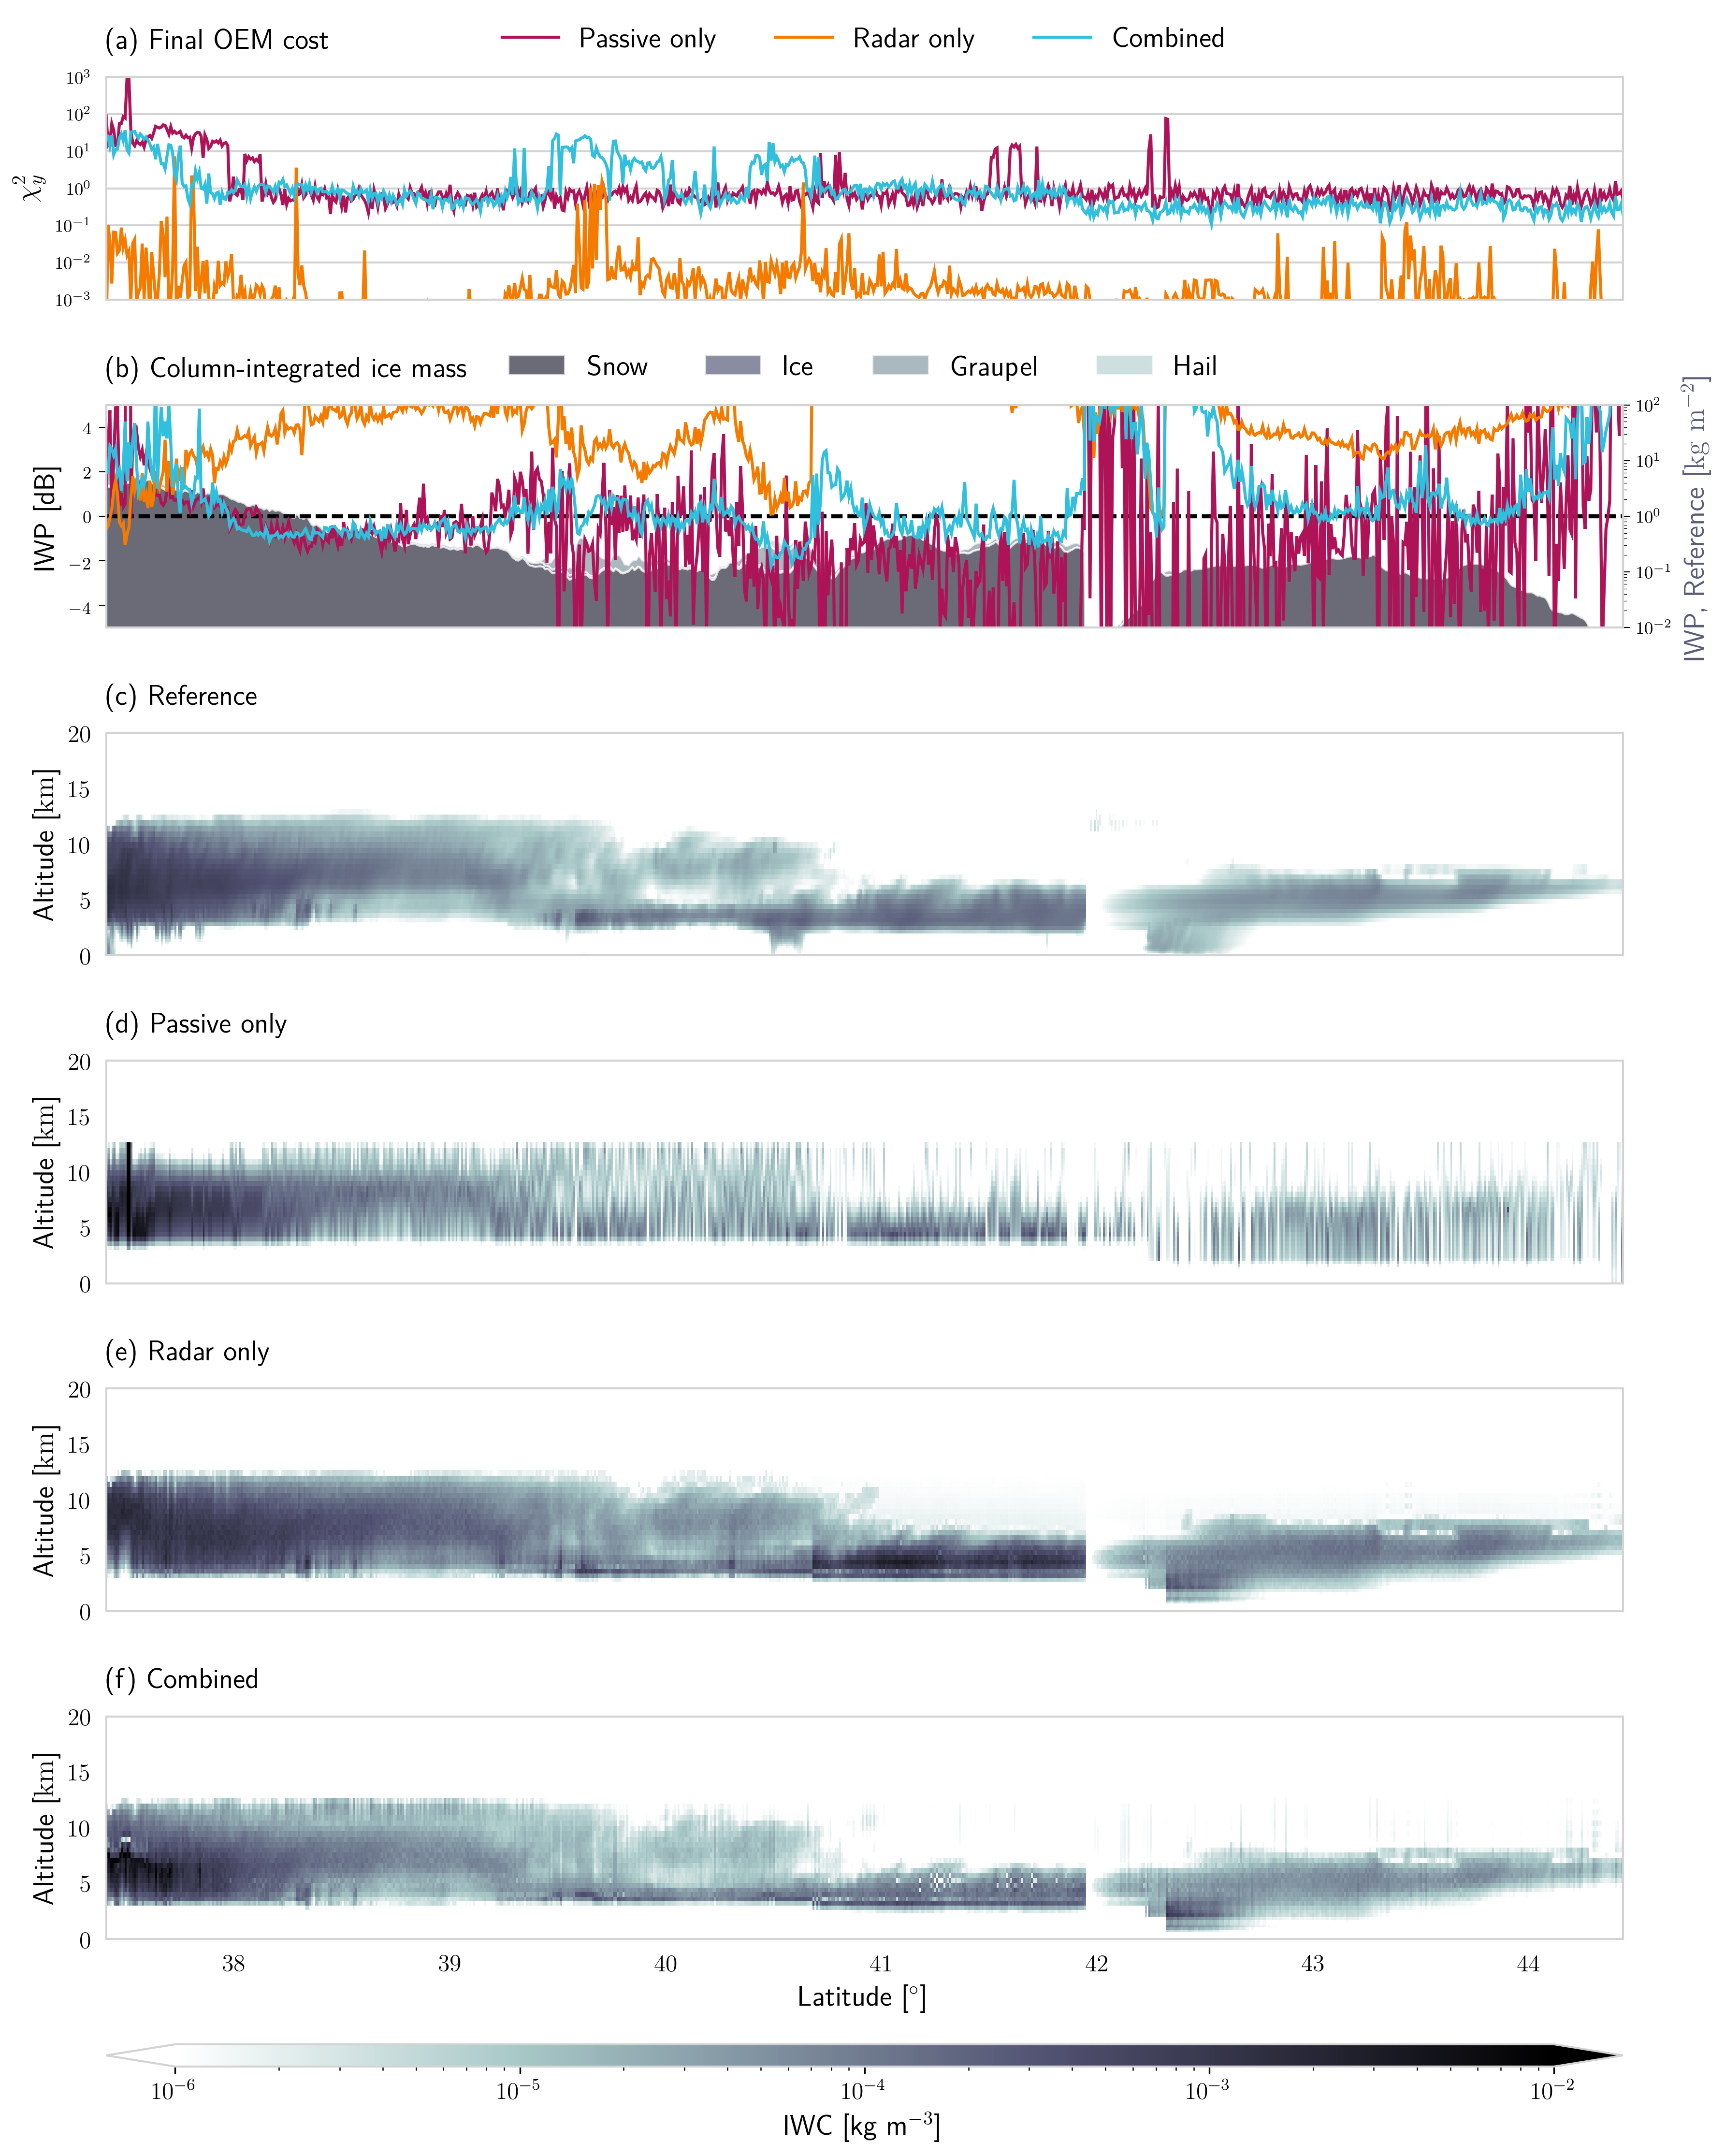
\includegraphics[width = 0.8\textwidth]{../plots/results_b_LargePlateAggregate}
\caption{Results of the ice hydrometeor retrieval for the second test scene.
  Panel (a) displays the value of the $\chi^2_y$ diagnostic normalized by the
  dimension of the measurement space of the corresponding retrieval. Panel (b)
  shows retrieved IWP in dB relative to the reference IWP. Reference IWP and the
  contributions from different hydrometeor classes are displayed by the filled
  areas in the background. Panel (c) displays the reference mass concentrations
  from the model scene. Panel (d), (e) and (f) display the retrieval results for
  the passive-only, radar-only and combined retrieval, respectively.}
\label{fig:results_b}
\end{figure}

\begin{figure}[!h]
\centering
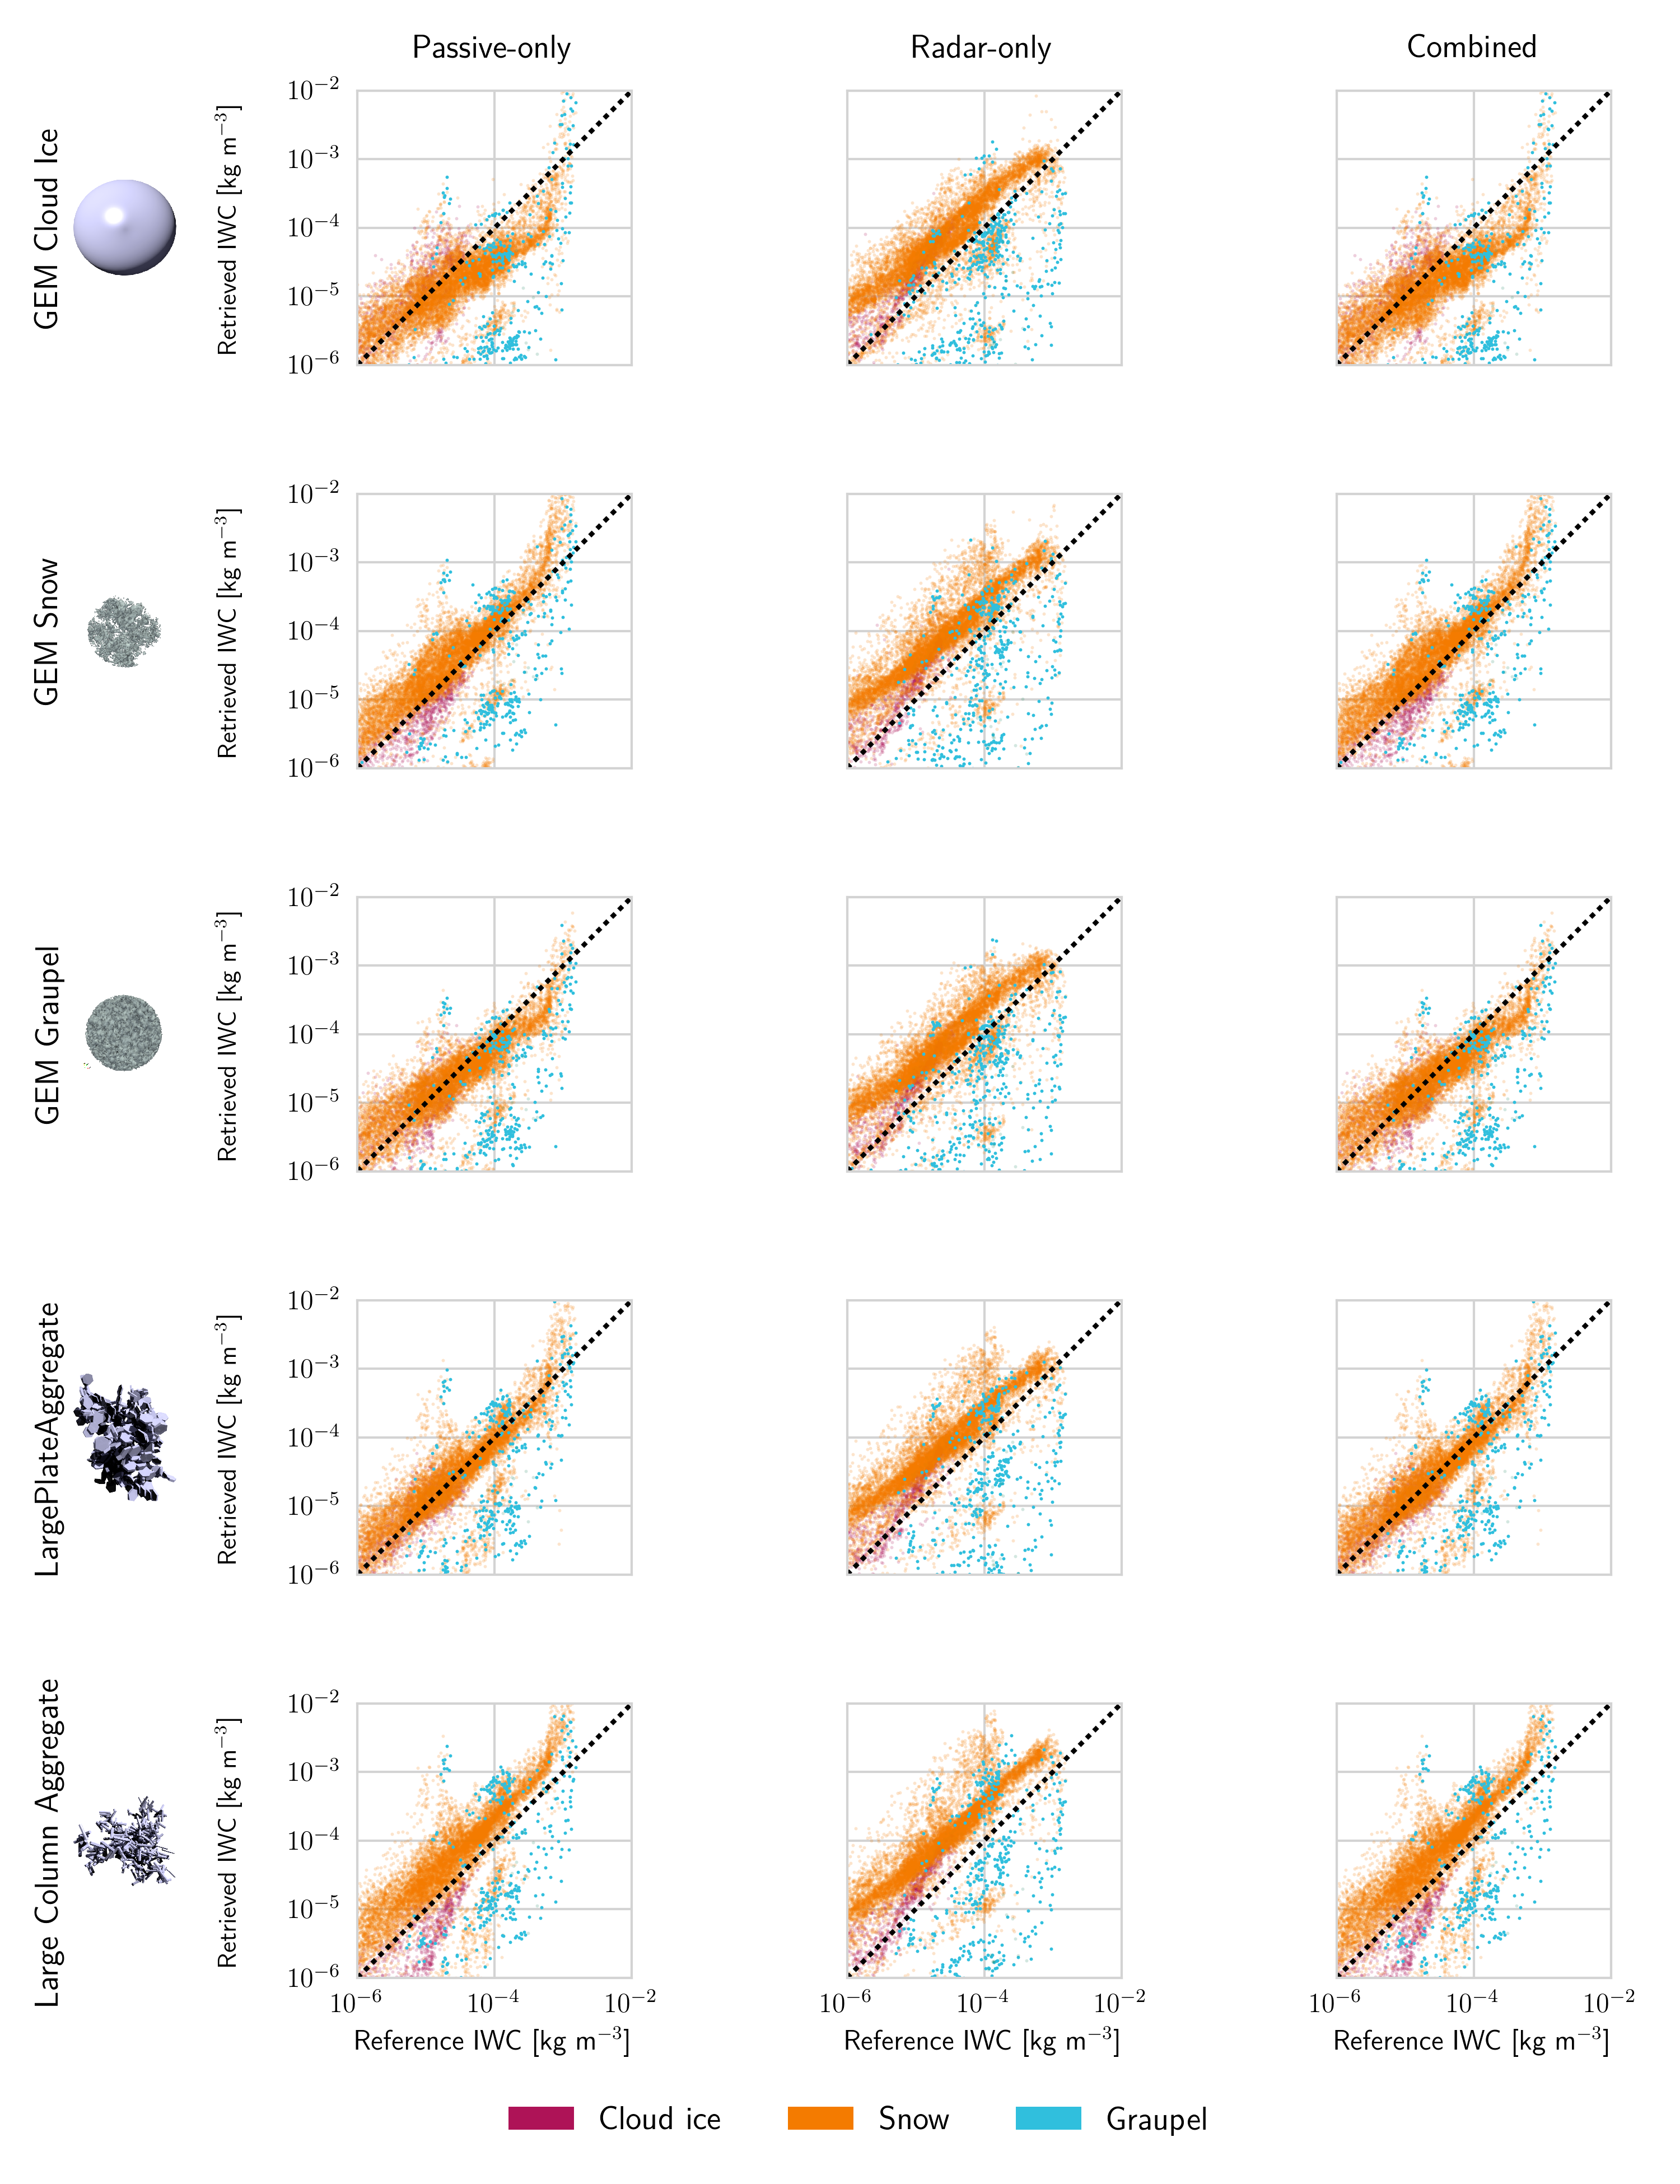
\includegraphics[width = 0.8\textwidth]{../plots/results_scatter_b}
\caption{Scatter plots of the reference and retrieved IWC for
  the second test scene. The rows show the retrieval results for a given
  assumed ice particle model. The first column of each row displays a rendering
  of the particle model. The following rows display the results for the
  passive-only, the radar-only and the combined retrieval.}
\label{fig:results_scatter_b}
\end{figure}

\clearpage


%% Please add \clearpage between each table and/or figure. Further guidelines on figures and tables can be found below.

\noappendix


\authorcontribution{Simon Pfreundschuh has implemented the retrieval, performed
  the data analysis and written the manuscript. Patrick Eriksson and Richard
  Larsson have added code to the ARTS radiative transfer model that was required
  to perform the presented calculations. Stefan A. Buehler, Patrick Eriksson,
  Manfred Brath and Simon Pfreundschuh have collaborated on the study that lead
  to the results presented here. David Duncan and Robin Ekelund have contributed
  to the conceptualization of the study through comments and advice.}



\competinginterests{No competing interests are present.} %% this section is mandatory even if you declare that no competing interests are present

\begin{acknowledgements}

The combined and radar-only were developed as part of the ESA-funded study
``Scientific Concept Study for Wide-Swath High-Resolution Cloud Profiling''
(Contract number: 4000119850/17/NL/LvH). The authors would like to thank
study manager Tobias Wehr for his valuable input and guidance.

Furthermore, the authors would like to acknowledge the work of Zhipeng Qu,
Howard Barker, and Jason Cole from Environment and Climate Change Canada who
produced the model scenes that were used to test the retrieval.

The work of SP, PE and RE on this study was financially supported by the Swedish
National Space Agency (SNSA) under grants 150/14 and 166/18.

SB is contributing to the Center for Earth System Research and Sustainability
(CEN) of Universit\"{a}t Hamburg.

The computations for this study were performed using several freely available programming
languages and software packages, most prominently the Python language
\citep{python}, the IPython computing environment \citep{ipython}, the numpy
package for numerical computing \citep{numpy} and matplotlib for generating
figures \citep{matplotlib}.

The computations were performed on resources at Chalmers Centre for
Computational Science and Engineering (C3SE) provided by the Swedish National
Infrastructure for Computing (SNIC).

\end{acknowledgements}




%% REFERENCES

%% The reference list is compiled as follows:


%% Since the Copernicus LaTeX package includes the BibTeX style file copernicus.bst,
%% authors experienced with BibTeX only have to include the following two lines:

\bibliographystyle{copernicus}
\bibliography{references}
%%
%% URLs and DOIs can be entered in your BibTeX file as:
%%
%% URL = {http://www.xyz.org/~jones/idx_g.htm}
%% DOI = {10.5194/xyz}


%% LITERATURE CITATIONS
%%
%% command                        & example result
%% \citet{jones90}|               & Jones et al. (1990)
%% \citep{jones90}|               & (Jones et al., 1990)
%% \citep{jones90,jones93}|       & (Jones et al., 1990, 1993)
%% \citep[p.~32]{jones90}|        & (Jones et al., 1990, p.~32)
%% \citep[e.g.,][]{jones90}|      & (e.g., Jones et al., 1990)
%% \citep[e.g.,][p.~32]{jones90}| & (e.g., Jones et al., 1990, p.~32)
%% \citeauthor{jones90}|          & Jones et al.
%% \citeyear{jones90}|            & 1990



%% FIGURES

%% When figures and tables are placed at the end of the MS (article in one-column style), please add \clearpage
%% between bibliography and first table and/or figure as well as between each table and/or figure.


%% ONE-COLUMN FIGURES

%%f
%\begin{figure}[t]
%\includegraphics[width=8.3cm]{FILE NAME}
%\caption{TEXT}
%\end{figure}
%
%%% TWO-COLUMN FIGURES
%
%%f
%\begin{figure*}[t]
%\includegraphics[width=12cm]{FILE NAME}
%\caption{TEXT}
%\end{figure*}
%
%
%%% TABLES
%%%
%%% The different columns must be seperated with a & command and should
%%% end with \\ to identify the column brake.
%
%%% ONE-COLUMN TABLE
%
%%t
%\begin{table}[t]
%\caption{TEXT}
%\begin{tabular}{column = lcr}
%\tophline
%
%\middlehline
%
%\bottomhline
%\end{tabular}
%\belowtable{} % Table Footnotes
%\end{table}
%
%%% TWO-COLUMN TABLE
%
%%t
%\begin{table*}[t]
%\caption{TEXT}
%\begin{tabular}{column = lcr}
%\tophline
%
%\middlehline
%
%\bottomhline
%\end{tabular}
%\belowtable{} % Table Footnotes
%\end{table*}
%
%%% LANDSCAPE TABLE
%
%%t
%\begin{sidewaystable*}[t]
%\caption{TEXT}
%\begin{tabular}{column = lcr}
%\tophline
%
%\middlehline
%
%\bottomhline
%\end{tabular}
%\belowtable{} % Table Footnotes
%\end{sidewaystable*}
%
%
%%% MATHEMATICAL EXPRESSIONS
%
%%% All papers typeset by Copernicus Publications follow the math typesetting regulations
%%% given by the IUPAC Green Book (IUPAC: Quantities, Units and Symbols in Physical Chemistry,
%%% 2nd Edn., Blackwell Science, available at: http://old.iupac.org/publications/books/gbook/green_book_2ed.pdf, 1993).
%%%
%%% Physical quantities/variables are typeset in italic font (t for time, T for Temperature)
%%% Indices which are not defined are typeset in italic font (x, y, z, a, b, c)
%%% Items/objects which are defined are typeset in roman font (Car A, Car B)
%%% Descriptions/specifications which are defined by itself are typeset in roman font (abs, rel, ref, tot, net, ice)
%%% Abbreviations from 2 letters are typeset in roman font (RH, LAI)
%%% Vectors are identified in bold italic font using \vec{x}
%%% Matrices are identified in bold roman font
%%% Multiplication signs are typeset using the LaTeX commands \times (for vector products, grids, and exponential notations) or \cdot
%%% The character * should not be applied as mutliplication sign
%
%
%%% EQUATIONS
%
%%% Single-row equation
%
%\begin{equation}
%
%\end{equation}
%
%%% Multiline equation
%
%\begin{align}
%& 3 + 5 = 8\\
%& 3 + 5 = 8\\
%& 3 + 5 = 8
%\end{align}
%
%
%%% MATRICES
%
%\begin{matrix}
%x & y & z\\
%x & y & z\\
%x & y & z\\
%\end{matrix}
%
%
%%% ALGORITHM
%
%\begin{algorithm}
%\caption{...}
%\label{a1}
%\begin{algorithmic}
%...
%\end{algorithmic}
%\end{algorithm}
%
%
%%% CHEMICAL FORMULAS AND REACTIONS
%
%%% For formulas embedded in the text, please use \chem{}
%
%%% The reaction environment creates labels including the letter R, i.e. (R1), (R2), etc.
%
%\begin{reaction}
%%% \rightarrow should be used for normal (one-way) chemical reactions
%%% \rightleftharpoons should be used for equilibria
%%% \leftrightarrow should be used for resonance structures
%\end{reaction}
%
%
%%% PHYSICAL UNITS
%%%
%%% Please use \unit{} and apply the exponential notation


\end{document}
